\chapter[Teoría de Amplificadores de Potencia]{Teoría de Amplificadores de Potencia} \label{sec:teoria_pa}
Los amplificadores de potencia (Power Amplifiers, PA) constituyen una etapa de la cadena de transmisión de un sistema de comunicaciones por radiofrecuencia. Su función es incrementar el nivel de potencia de una señal de RF hasta un valor suficiente para su transmisión, proporcionando la potencia necesaria a la carga, típicamente una antena, a partir de la potencia suministrada por una fuente de alimentación de continua. Debido a que esta etapa procesa los niveles más elevados de potencia del transmisor, su desempeño tiene un impacto directo sobre el consumo energético, la autonomía del sistema y la calidad de la señal transmitida.

En el caso ideal, un amplificador de potencia amplifica la señal de entrada sin modificar su forma de onda. Al mismo tiempo, toda la potencia de continua suministrada por la fuente debe convertirse en potencia útil de RF, minimizando la potencia disipada en forma de calor. Es decir, el caso ideal presenta una eficiencia del 100\,\%. Este aspecto resulta particularmente importante en aplicaciones espaciales, donde la potencia disponible y la capacidad de disipación térmica son recursos limitados.

Sin embargo, este comportamiento no puede alcanzarse en dispositivos reales. El transistor, como elemento activo, presenta una característica de transferencia inherentemente no lineal, cuya respuesta depende tanto de las condiciones de polarización como del nivel de excitación. Como consecuencia, parte de la potencia suministrada se disipa en forma de calor y la señal de salida experimenta distintos tipos de distorsión, tales como compresión de ganancia, generación de armónicos y productos de intermodulación. Estas limitaciones impiden maximizar simultáneamente la potencia de salida, la eficiencia y la linealidad del amplificador. En consecuencia, el diseño de un amplificador de potencia consiste en encontrar un compromiso adecuado entre estas prestaciones, de acuerdo con los requerimientos de la aplicación.

En este capítulo se presentan los fundamentos teóricos necesarios para el diseño de amplificadores de potencia de RF. En primer lugar se analiza el principio de funcionamiento de los amplificadores de potencia y la influencia del ángulo de conducción sobre las distintas clases de operación, estableciendo la relación entre eficiencia, potencia de salida y contenido armónico. Posteriormente se introducen los parámetros de pequeña y gran señal empleados para caracterizar el desempeño del amplificador, así como las principales métricas de linealidad utilizadas en aplicaciones de comunicaciones. Finalmente, se describen los conceptos de adaptación de impedancias y el método de \textit{load-pull}, herramienta fundamental para la determinación de la impedancia óptima de carga en el diseño de amplificadores de potencia.

% -----------------------------------------------------------------------------------------------%
\section{Funcionamiento y clases de operación} \label{sec:funcionamiento_clases}
La Figura~\ref{fig:pa_topology} muestra el esquema simplificado de un amplificador de potencia de RF de una sola etapa basado en un transistor MOS de canal N. La señal de entrada se aplica al gate del transistor a través de un capacitor de acople (\textit{DC block}), el cual impide el paso de la componente continua de polarización mientras permite el paso de la señal de radiofrecuencia. De manera análoga, un segundo capacitor desacopla la tensión continua presente en el drain de la carga conectada a la salida.

La alimentación de continua se suministra al drain mediante un choke de RF, quien presenta una impedancia prácticamente nula para la componente continua, permitiendo la circulación de la corriente de alimentación, mientras que ofrece una elevada impedancia a la frecuencia de operación, evitando que la potencia de RF se derive hacia la alimentación.

Finalmente, la red resonante formada por el inductor y el capacitor en derivación se encuentra sintonizada a la frecuencia fundamental de operación. En resonancia, esta red presenta una elevada impedancia, permitiendo el desarrollo de la tensión correspondiente a la componente fundamental sobre la carga \(R_L\). Para las componentes armónicas, en cambio, la impedancia de la red disminuye considerablemente, proporcionando un camino de baja impedancia hacia masa que atenúa dichas componentes. Como resultado, la tensión presente sobre la carga es aproximadamente senoidal aun cuando la corriente generada por el transistor contenga un importante contenido armónico. En otras palabras, el paralelo LC actúa como filtro pasabanda sintonizado a la frecuencia fundamental de la señal.

\begin{figure}
    \centering
    \begin{tikzpicture}[transform shape]
        % Paths, nodes and wires:
        \node[nigfete] at (7, 4.27){};
        \draw (3.25, 4) to[capacitor, l={$DC \, Block$}] (4.5, 4);
        \draw (7.5, 5) to[capacitor, l={$DC \, Block$}] (8.75, 5);
        \draw (5.5, 2.25) to[cute choke, l={$RF \, Choke$}, label distance=0.03cm] (5.5, 3.75);
        \draw (7, 5.25) to[cute choke, l={$RF \, Choke$}, label distance=0.03cm] (7, 6.75);
        \draw (5, 4) -- (6, 4) |- (5.5, 4) -| (5.5, 3.75);
        \draw (5.5, 2.25) to[battery1, l={$V_{GG}$}] (5.5, 1.25);
        \node[oscillator](N1) at (2.74, 3.01){} node[anchor=east] at ([xshift=-0.03cm]N1.west){$v_{in}$};
        \draw (2.25, 2.5) -| (2.25, 1);
        \node[tlground] at (2.25, 1){};
        \node[tlground] at (5.5, 1){};
        \node[tlground] at (7, 1){};
        \draw (7, 3.5) -- (7, 1);
        \draw (11.75, 4.5) to[american resistor, /tikz/circuitikz/bipoles/length=1.26cm, l={$R_L$}] (11.75, 2.5);
        \node[tlground] at (9.25, 1){};
        \draw (14, 6.25) to[battery1, l={$V_{DD}$}] (14, 5.25);
        \draw (14, 5.25) -| (14, 1);
        \node[tlground] at (14, 1){};
        \draw (7, 5.25) -| (7, 5.04);
        \draw (7, 5) -- (7.5, 5);
        \draw (8.75, 5) -- (9.25, 5) -| (9.25, 4.5);
        \draw (7, 6.75) -- (7, 7) -- (14, 7) -- (14, 6.25);
        \draw (2.25, 4) -| (2.25, 3.5);
        \draw (2.25, 4) -- (3.25, 4);
        \draw (4.5, 4) -- (5, 4);
        \draw (5.5, 1.25) -| (5.5, 1);
        \draw (10.5, 3) to[capacitor, l_={$C$}] (10.5, 4);
        \draw (9.25, 4.25) to[cute inductor, mirror, l={$L$}, label distance=-0.04cm] (9.25, 2.75);
        \draw (9.25, 4.5) -| (9.25, 4.25);
        \draw (9.25, 5) -- (10.5, 5) -| (10.5, 4);
        \draw (10.5, 3) -| (10.5, 1);
        \draw (9.25, 2.75) -| (9.25, 1);
        \node[tlground] at (10.5, 1){};
        \draw (10.5, 5) -| (11.75, 4.5);
        \draw (11.75, 2.5) -| (11.75, 1);
        \node[tlground] at (11.75, 1){};
        \node[circ] at (10.5, 5){};
        \node[circ] at (9.25, 5){};
        \node[circ] at (5.5, 4){};
        \node[circ] at (7, 5){};
    \end{tikzpicture}
    \caption{Circuito simplificado de un amplificador.}
    \label{fig:pa_topology}
\end{figure}

A diferencia de los amplificadores de pequeña señal, un amplificador de potencia opera con niveles elevados de excitación, por lo que el transistor abandona la región estrictamente lineal de su característica de transferencia. En estas condiciones, la corriente de drain deja de ser proporcional a la tensión aplicada en gate y comienza a depender del intervalo durante el cual el dispositivo conduce corriente.

En un transistor NMOS, la conducción sólo tiene lugar cuando la tensión instantánea entre gate y source supera la tensión umbral del dispositivo. Si la señal de excitación posee una amplitud suficientemente elevada o el transistor se polariza próximo al corte, esta condición únicamente se verifica durante una fracción del período de la señal. Durante el resto del ciclo el transistor permanece apagado y la corriente de drain es prácticamente nula. El intervalo angular durante el cual existe conducción recibe el nombre de \textbf{ángulo de conducción} y se representa mediante \(\alpha\).

El valor del ángulo de conducción depende principalmente del punto de polarización elegido para el transistor. Si el dispositivo permanece conduciendo durante todo el ciclo de la señal, el ángulo de conducción es igual a \(360^\circ\) (\(2\pi\) rad). Al disminuir progresivamente la corriente de polarización, el transistor conduce durante una porción cada vez menor del período, reduciendo el valor de \(\alpha\). En consecuencia, la forma de onda de la corriente de drain deja de ser senoidal y adquiere la forma de pulsos de ancho decreciente. Suponiendo una señal de entrada senoidal, la corriente instantánea de drain puede expresarse como

\begin{equation}
    i_D(\theta)=
    \begin{cases}
        I_{max}\left(\dfrac{\cos\theta-\cos(\alpha/2)}{1-\cos(\alpha/2)}\right), & |\theta|\leq\dfrac{\alpha}{2} \\[2ex] 
        0, & |\theta|>\dfrac{\alpha}{2},
    \end{cases}
\label{eq:id_theta}
\end{equation}

donde \(I_{max}\) representa la corriente máxima de drenador y \(\theta=\omega t\) \cite[p.~41]{cripps2006}. 

En la Figura~\ref{fig:id_classes} se ilustran las formas de onda de la corriente de drain para las distintas clases de operación del amplificador.

\begin{figure}[H]
    \centering
    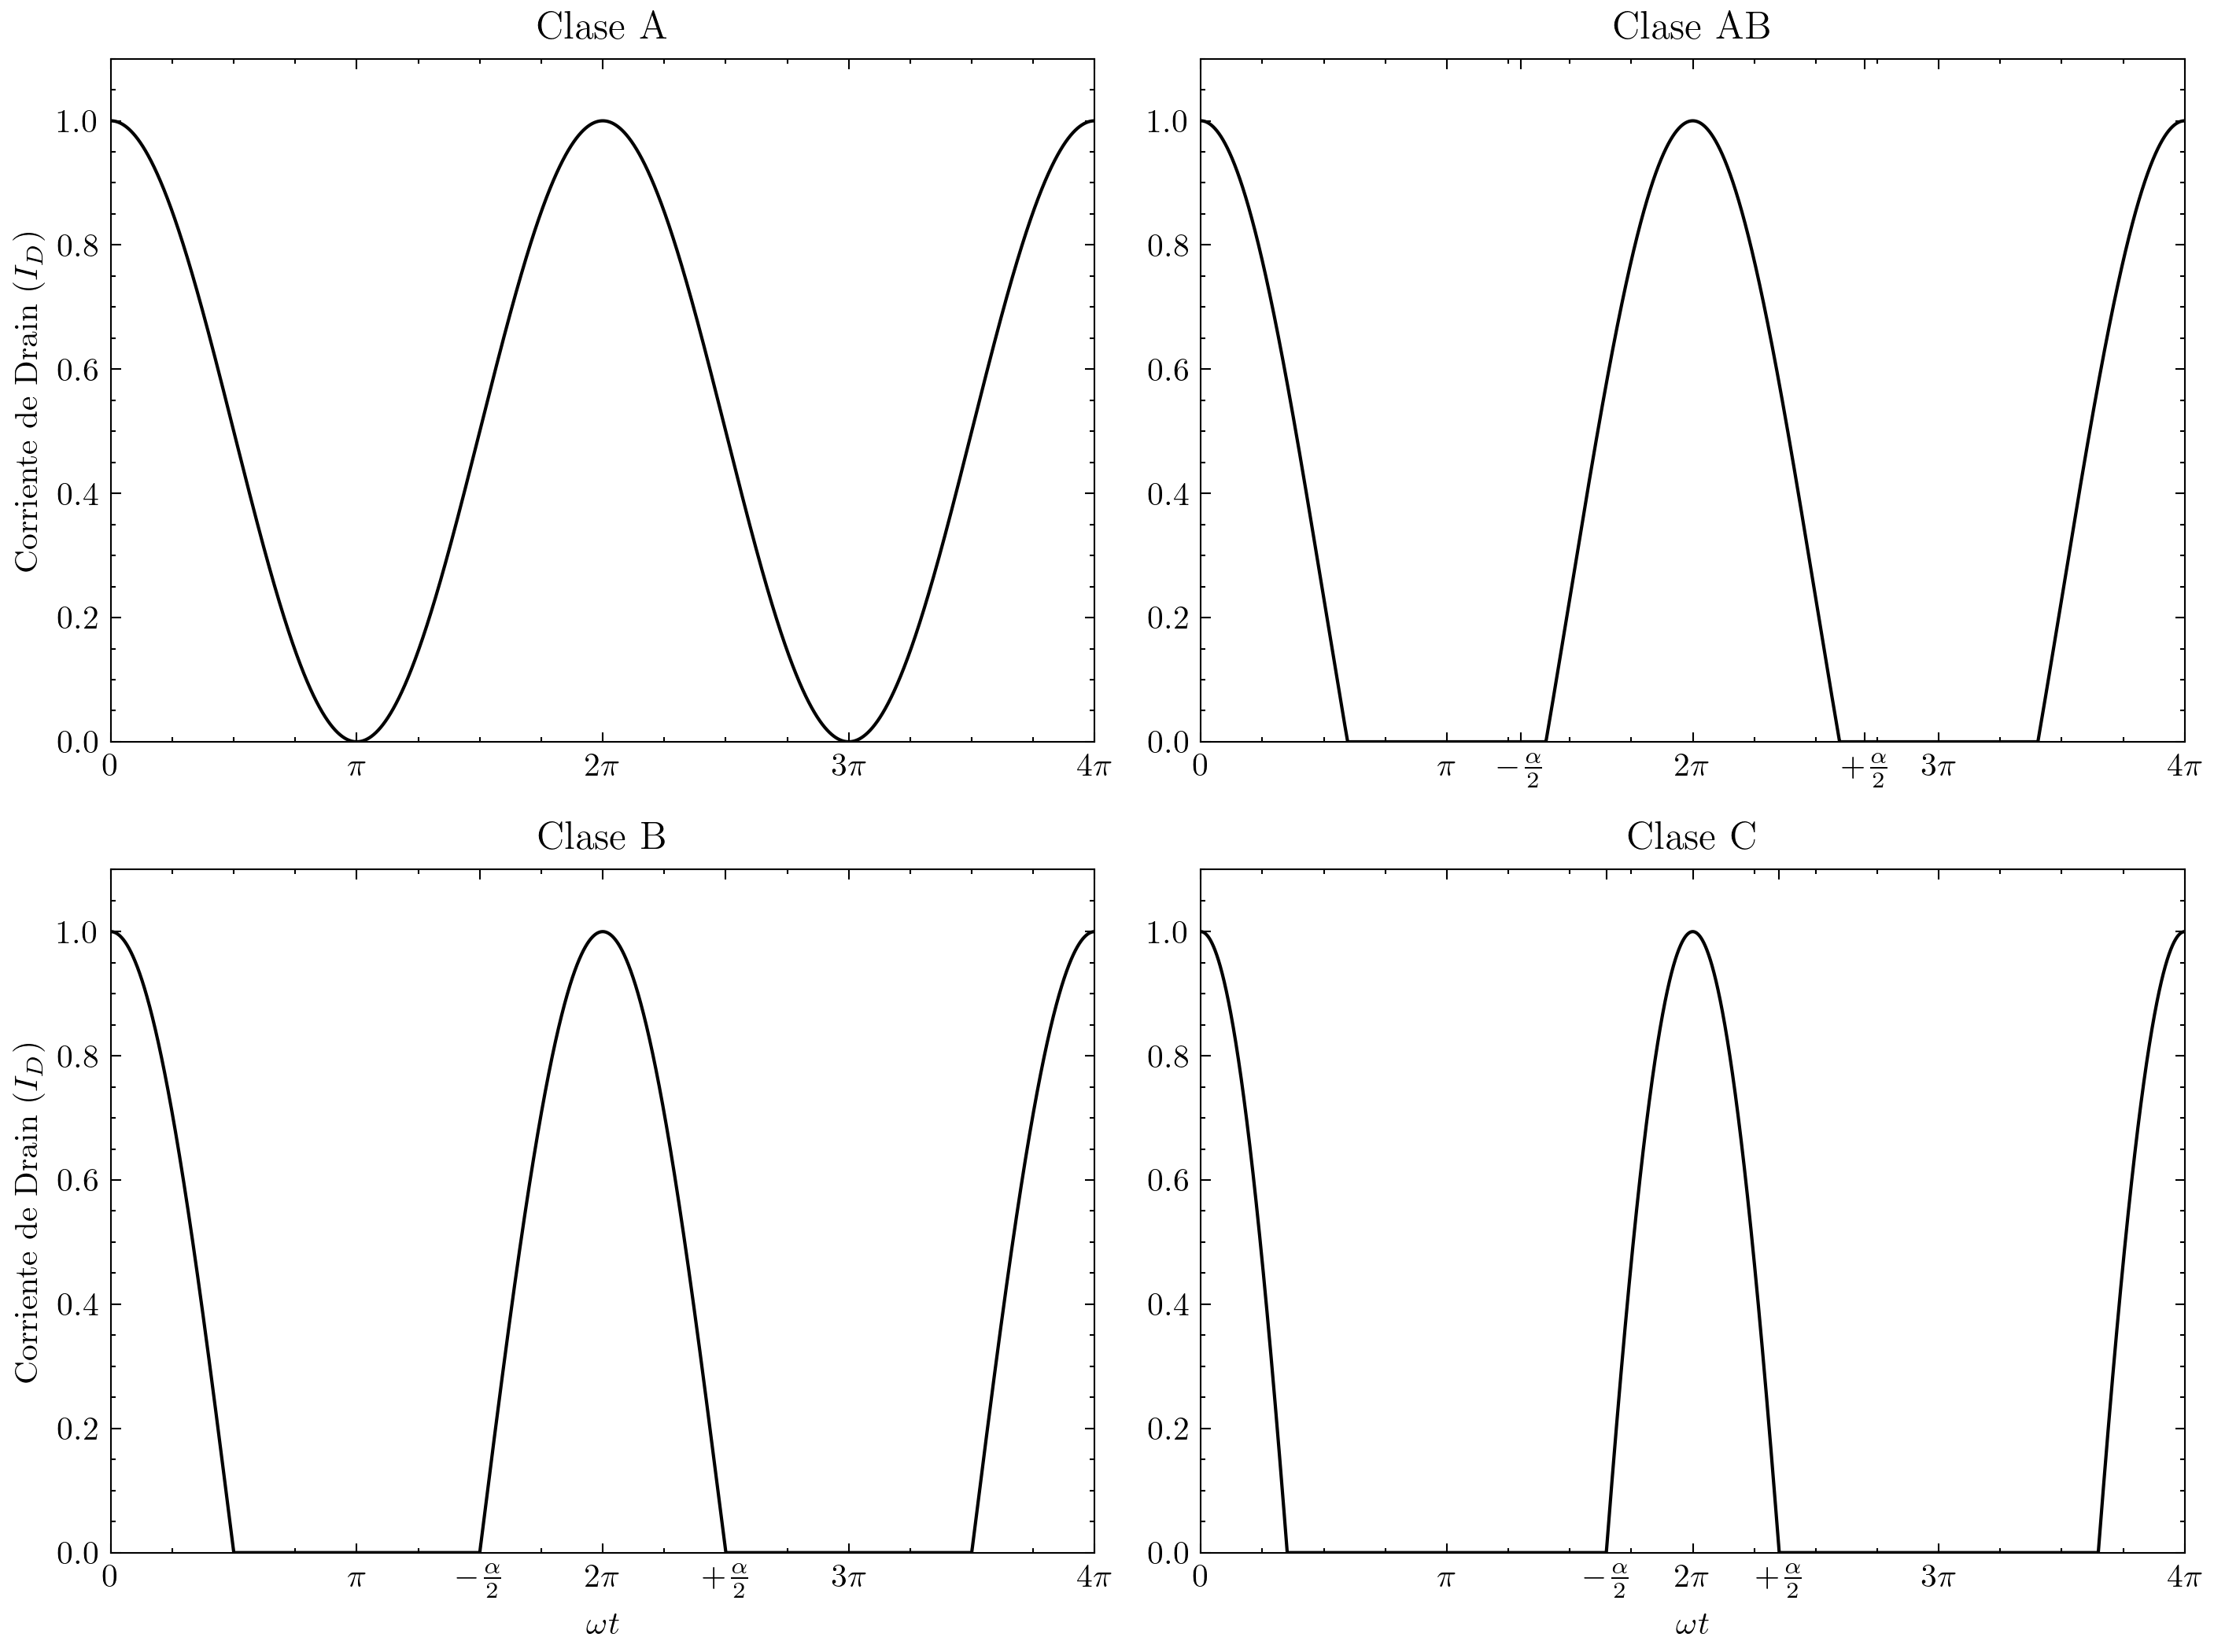
\includegraphics[width=\linewidth]{Figures/id_classes.png}
    \caption{Corrientes de drain para las distintas clases de operación de un amplificador suponiendo la debida polarización del circuito para cada caso.}
    \label{fig:id_classes}
\end{figure}

Al tratarse de una función periódica, la corriente puede desarrollarse mediante una serie de Fourier, obteniéndose una componente continua y un conjunto de componentes armónicas de la forma

\begin{equation}
i_D(\theta)= I_{DC} + \sum_{n=1}^{\infty}\,I_n\cos(n\theta)
\label{eq:fourier}
\end{equation}

siendo \(I_{DC}\) la componente continua e \(I_n\) la amplitud de la componente armónica de orden \(n\), obtenidas respectivamente mediante

\begin{equation}
    I_{DC} = \frac{1}{2\pi}\int_{-\alpha/2}^{\alpha/2} i_D(\theta)\,d\theta
    \label{eq:idc_generic}
\end{equation}

\begin{equation}
    I_n = \frac{1}{\pi}\int_{-\alpha/2}^{\alpha/2} i_D(\theta)\cos(n\theta)\,d\theta, \qquad n = 1, 2, 3, \dots
    \label{eq:in_generic}
\end{equation}

El análisis de estas componentes resulta interesante para poder relacionar el ángulo de conducción con la potencia disponible en la frecuencia fundamental, el contenido armónico de la corriente y la eficiencia. Asimismo, el valor de \(\alpha\) constituye el criterio utilizado para clasificar los amplificadores de potencia en las distintas clases de operación. En términos generales, un ángulo de conducción de \(360^\circ\) corresponde a un amplificador de clase A, mientras que valores comprendidos entre \(180^\circ\) y \(360^\circ\) dan lugar a la clase AB. Cuando el transistor conduce exactamente durante medio período se obtiene la clase B, y para ángulos inferiores a \(180^\circ\) se habla de operación en clase C \cite[p.~41]{cripps2006}.

La reducción del ángulo de conducción disminuye la potencia disipada en el dispositivo (al conducir por menos tiempo) y, por lo tanto, aumenta la eficiencia de conversión de potencia a la salida del transistor. Sin embargo, esta mejora se obtiene a costa de la pérdida de linealidad en la corriente de drain, aumentando el contenido armónico. Como consecuencia, ninguna clase de operación resulta simultáneamente óptima en cuanto a potencia de salida, eficiencia y linealidad.

La Figura~\ref{fig:armonicos_alpha} ilustra la amplitud normalizada de las primeras cinco componentes armónicas de la corriente de drain y el valor de la componente de continua en función del ángulo de conducción, evaluadas mediante la resolución de las ecuaciones~\eqref{eq:idc_generic} y \eqref{eq:in_generic}. Se observa que, a medida que el ángulo de conducción se reduce desde $\alpha = 360^\circ$ (Clase A) hacia valores progresivamente menores, la componente de continua $I_{DC}$ disminuye monótonamente, mientras que la componente fundamental $I_1$ se mantiene prácticamente constante en un amplio rango de valores de $\alpha$, alcanzando su máximo relativo en las proximidades de la Clase B, para luego decrecer también en el régimen de Clase C. Las componentes armónicas de orden superior ($I_2$ a $I_5$), prácticamente nulas en Clase A, adquieren magnitud creciente a medida que el ángulo de conducción se reduce, siendo esta aparición de armónicos la manifestación de la distorsión en la forma de onda de corriente.

\begin{figure}[H]
    \centering
    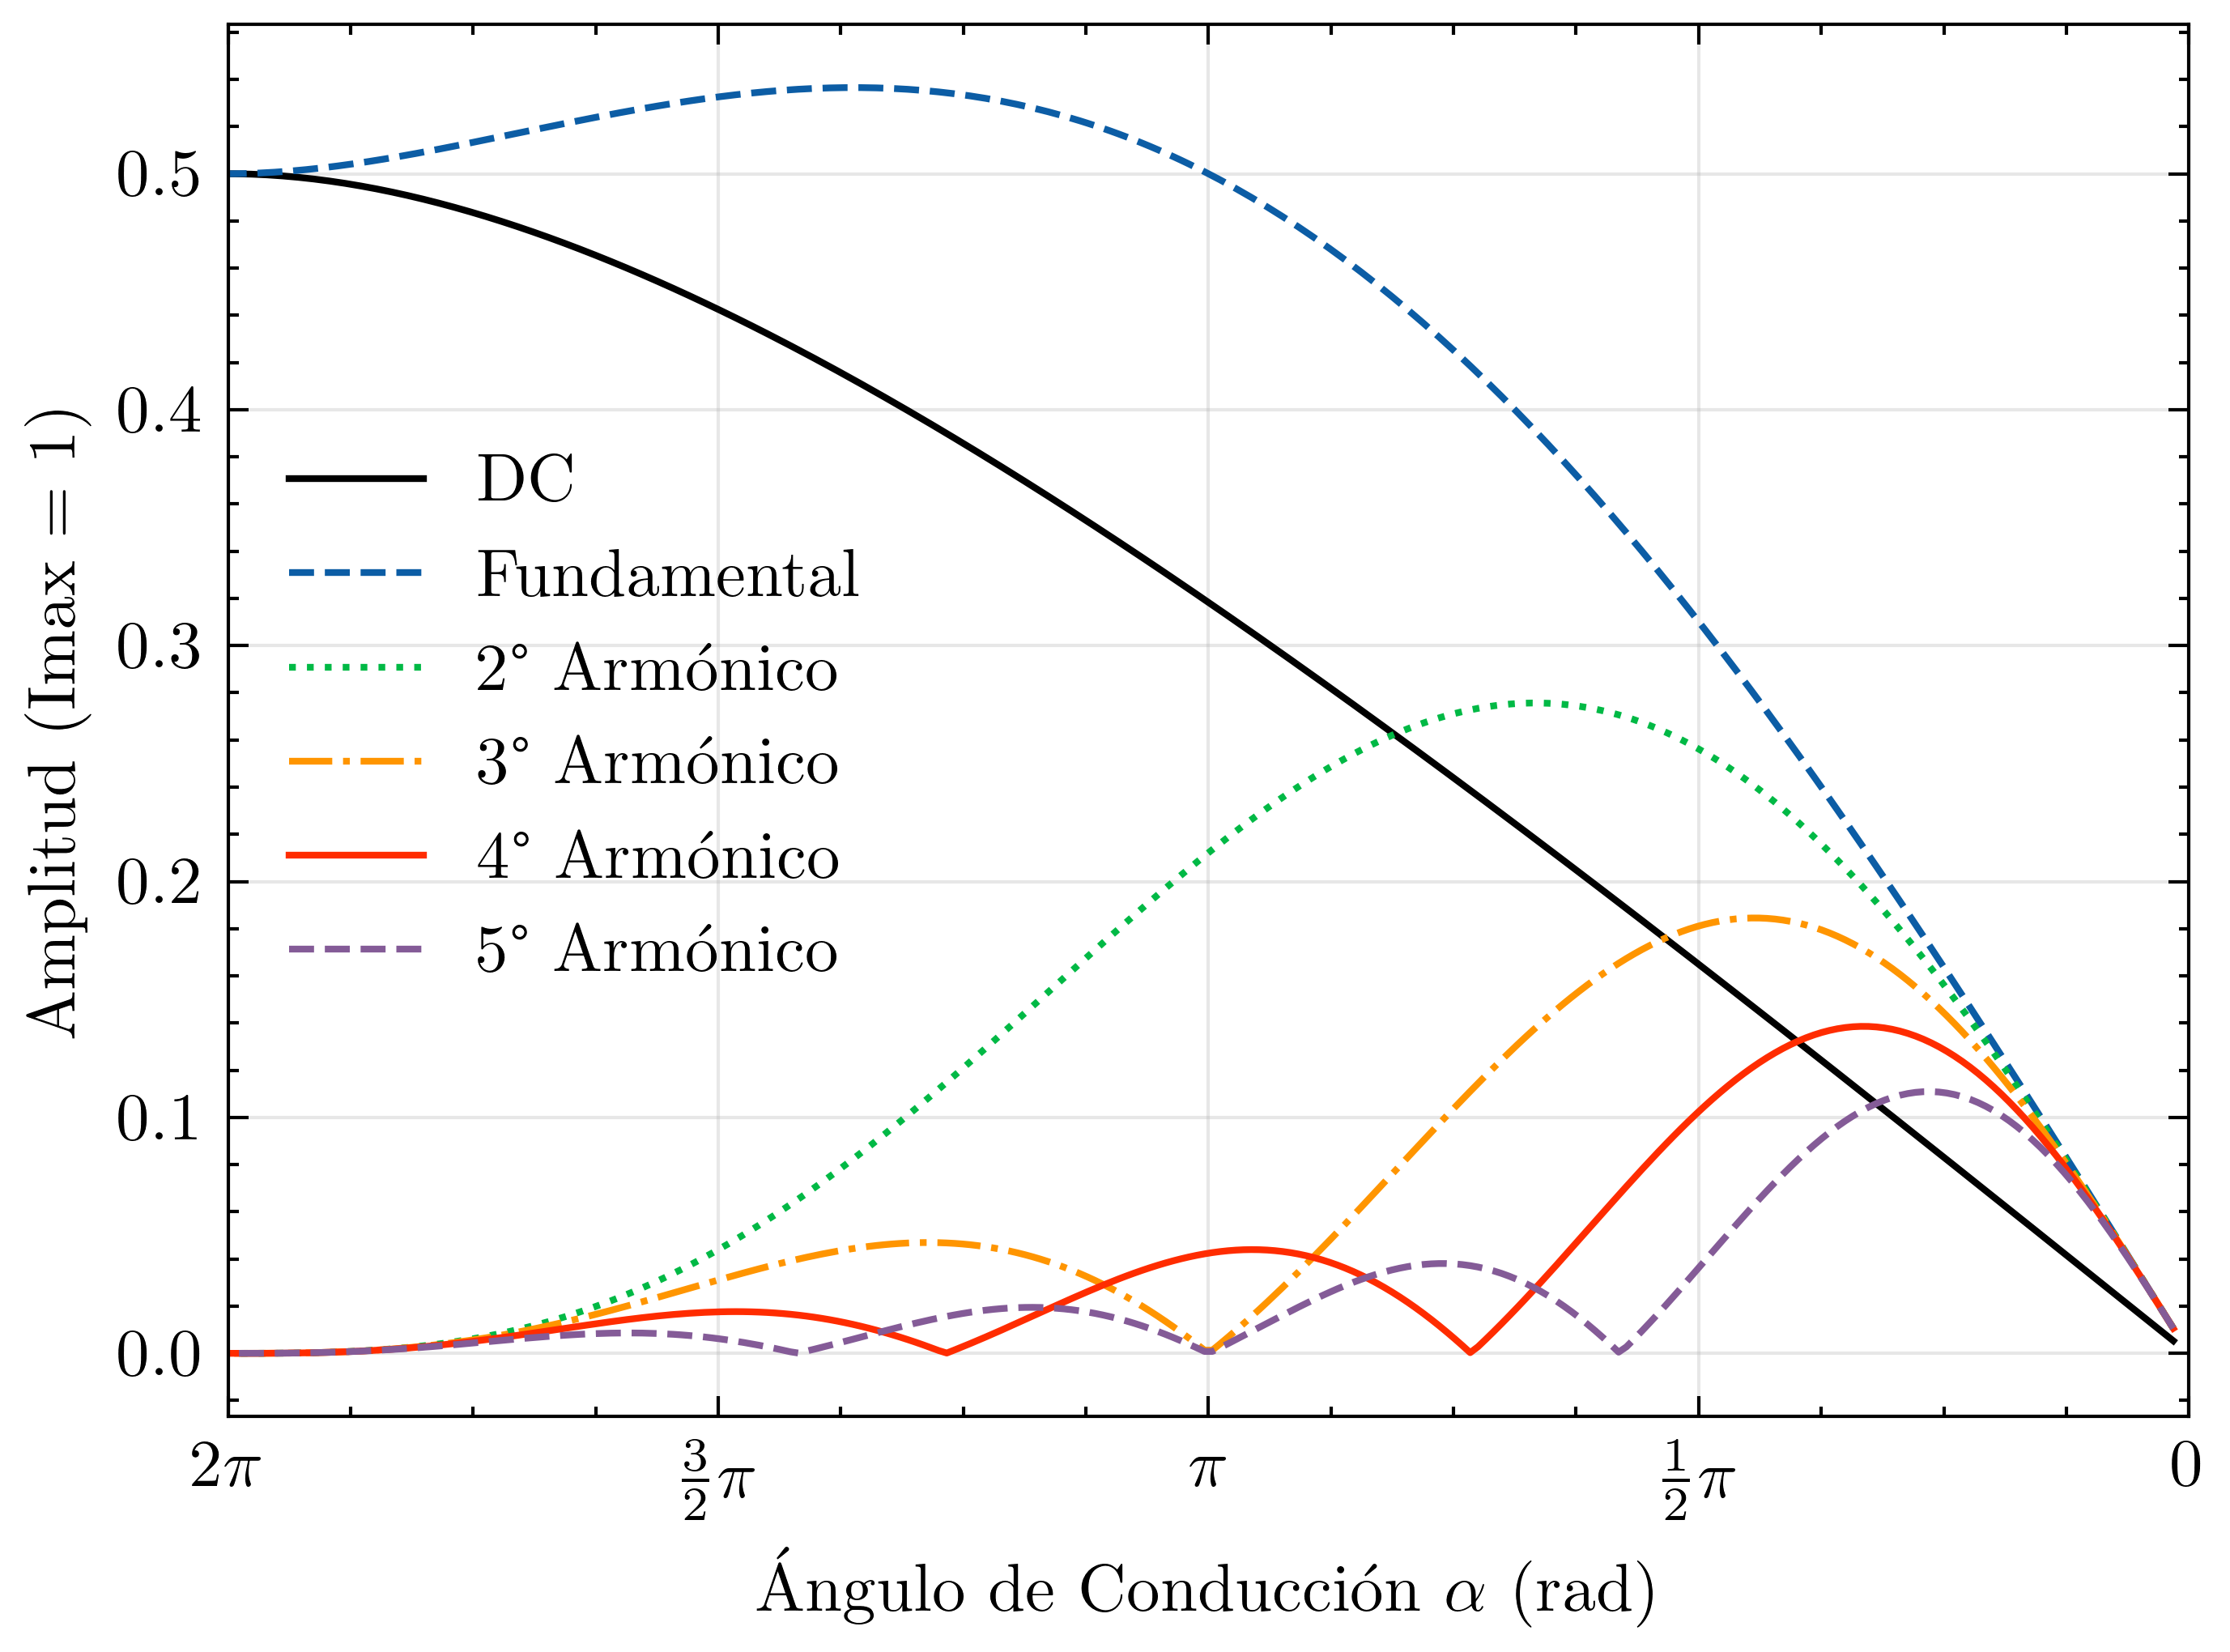
\includegraphics[width=\linewidth]{Figures/pa_harmonics.png}
    \caption{Amplitud normalizada de las componentes $I_{DC}$ a $I_5$ de la corriente de drain en función del ángulo de conducción $\alpha$.}
    \label{fig:armonicos_alpha}
\end{figure}

A partir de las componentes de continua y fundamental, la eficiencia de drain del amplificador, definida como el cociente entre la potencia de RF entregada a la carga y la potencia continua consumida, queda determinada en función del ángulo de conducción mediante la expresión \cite[p.~768]{razavi2011}

\begin{equation}
    \eta(\alpha) = \frac{1}{4}\,\frac{\alpha - \sin\alpha}{\sin(\alpha/2) - (\alpha/2)\cos(\alpha/2)}
    \label{eq:eficiencia_alpha}
\end{equation}

La Figura~\ref{fig:pa_efficiency} grafica la ecuación~\eqref{eq:eficiencia_alpha} para el rango completo de ángulos de conducción de interés, señalando la eficiencia correspondiente a cada clase de operación: $\eta = 50\%$ para la Clase A, $\eta \approx 78{,}5\%$ para la Clase B, valores intermedios entre ambos para la Clase AB, y valores crecientes por encima de este último para la Clase C, que tiende al $100\%$ en el límite de ángulo de conducción nulo. Este límite carece de sentido práctico, ya que implica ausencia total de conducción de corriente y potencia de salida nula.

\begin{figure}[H]
    \centering
    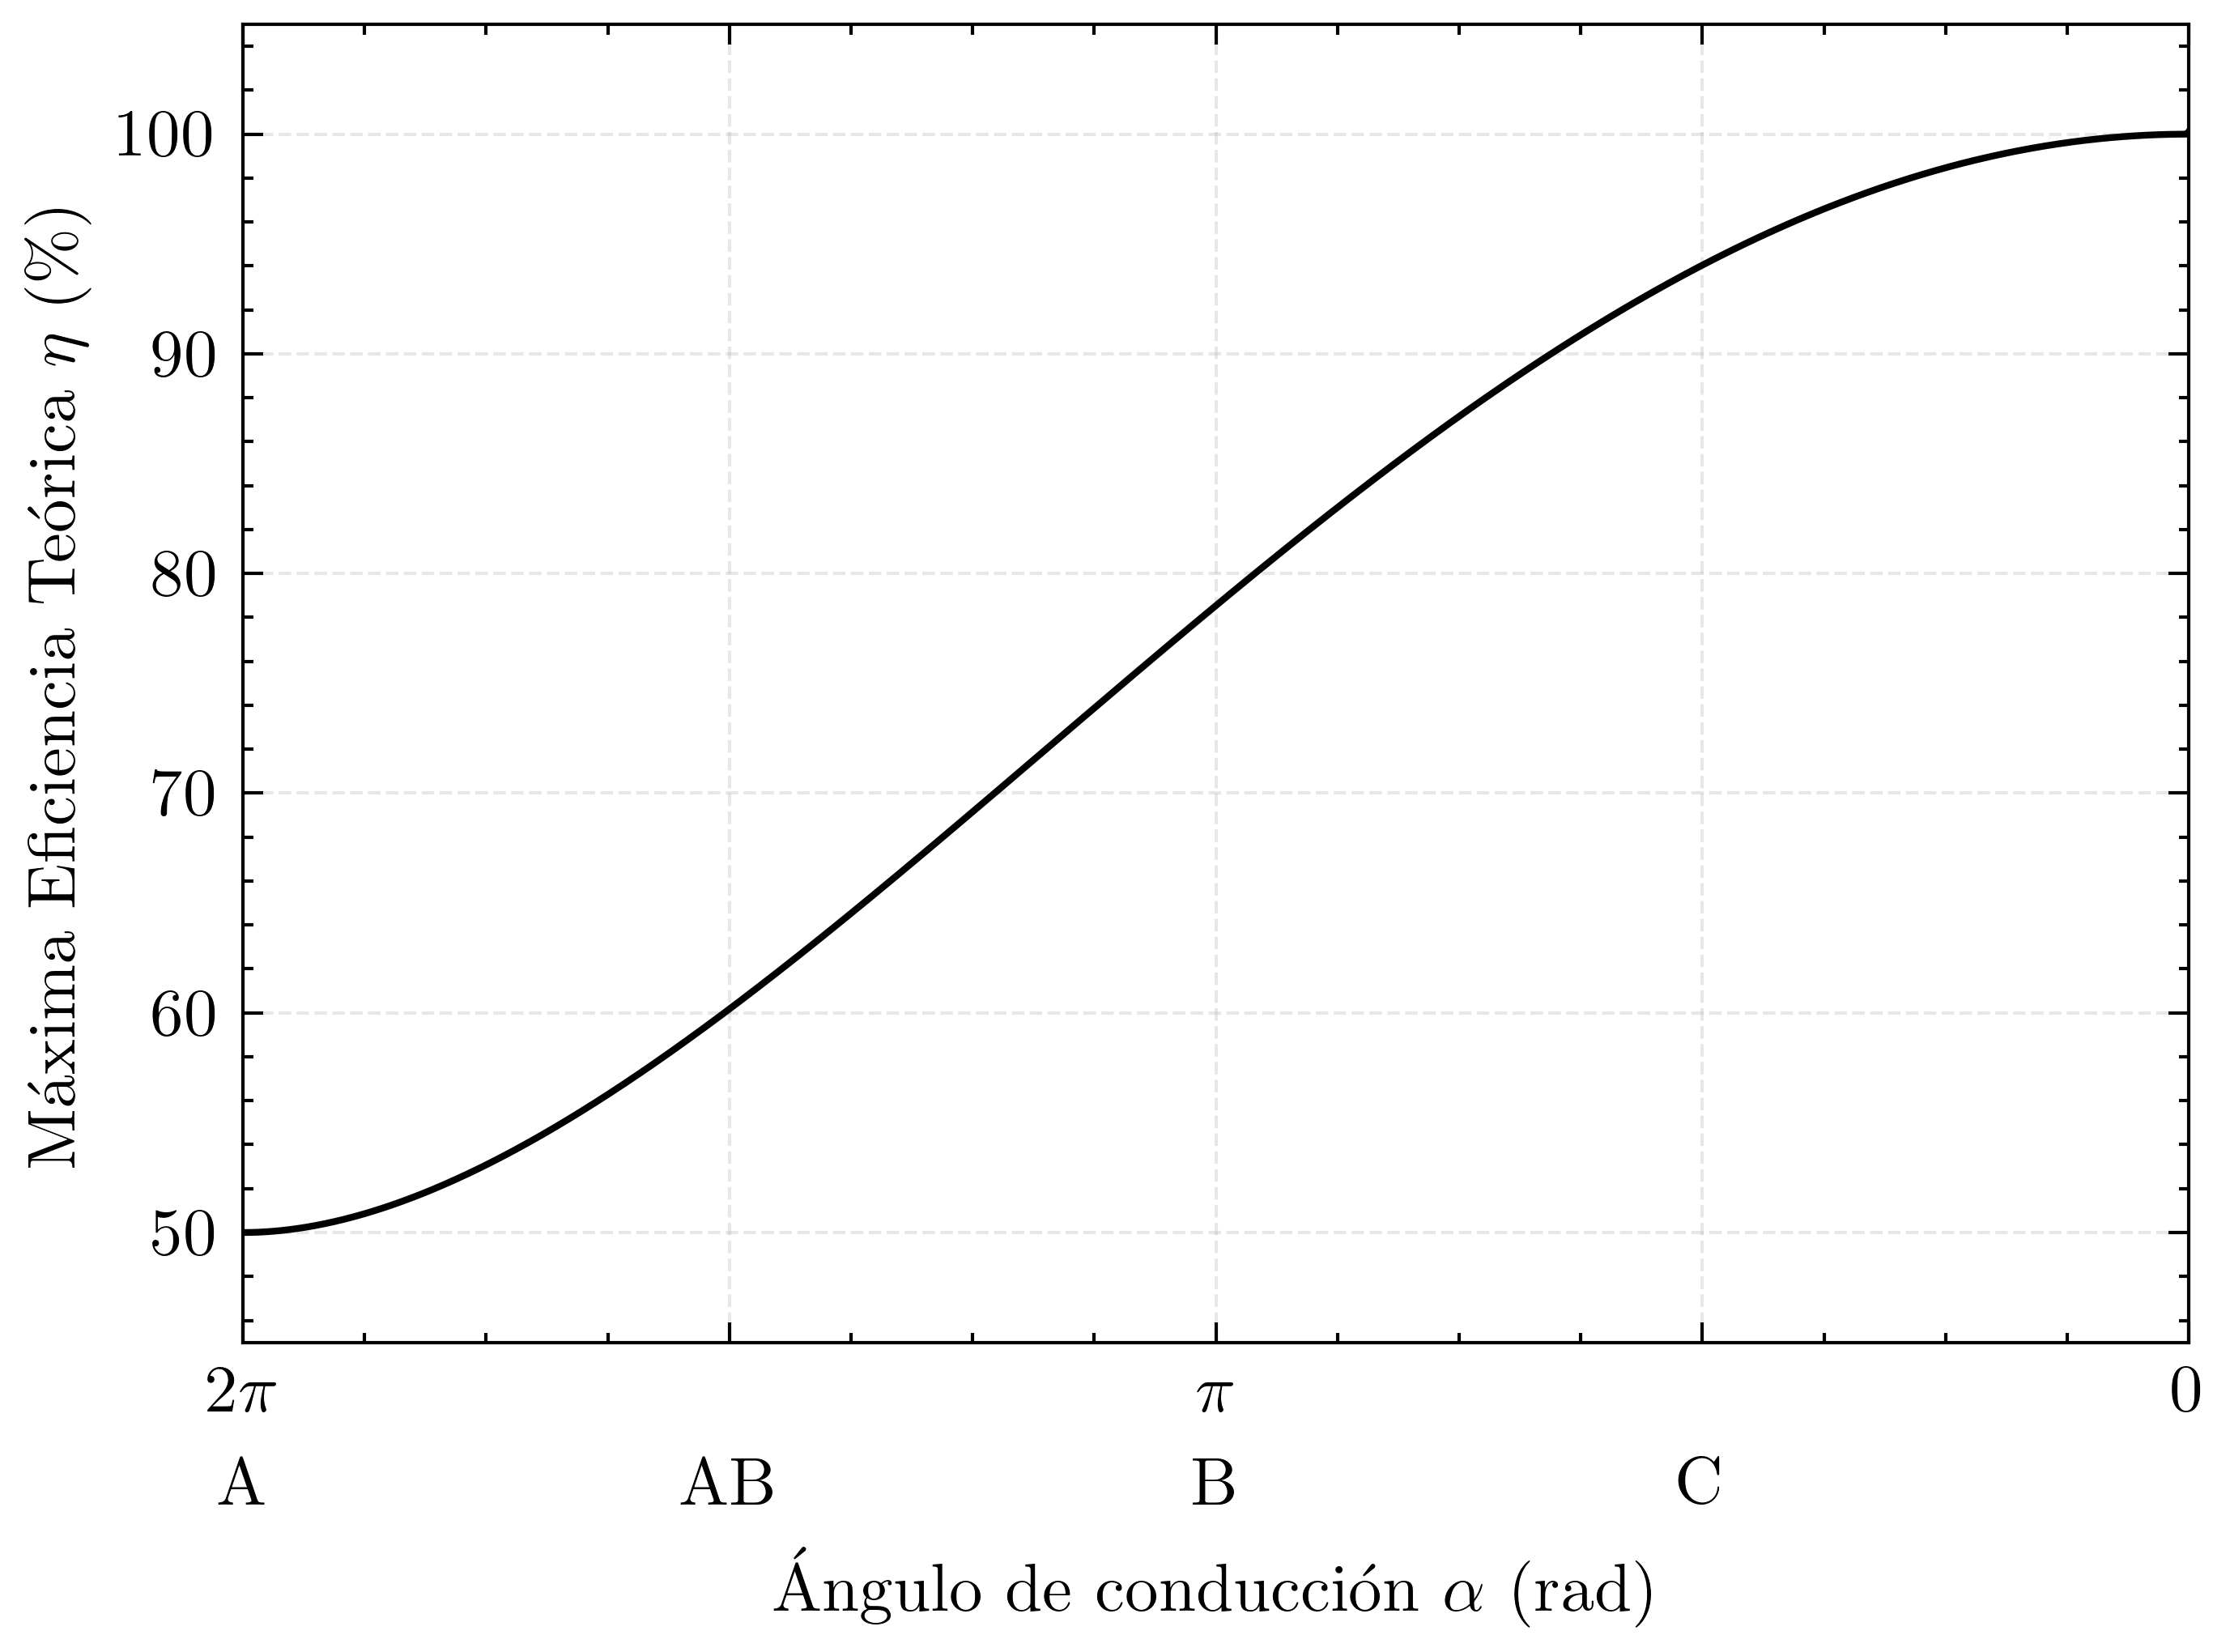
\includegraphics[width=\linewidth]{Figures/pa_efficiency.png}
    \caption{Eficiencia de drain teórica en función del ángulo de conducción, con las regiones correspondientes a las Clases A, AB, B y C señaladas.}
    \label{fig:pa_efficiency}
\end{figure}

La Figura~\ref{fig:rf_power_alpha} ilustra, en función del ángulo de conducción, la potencia de RF entregada a la carga referida a su valor en Clase A y evaluada asumiendo carga óptima y armónicos filtrados. Se observa que la potencia de RF permanece prácticamente constante, con una leve mejora, en el tramo comprendido entre la Clase A y la Clase B, tramo que coincide con el crecimiento inicial de $I_1$ señalado en la Figura~\ref{fig:armonicos_alpha}. Por debajo de la Clase B, en cambio, la potencia de RF decae de manera pronunciada a medida que el ángulo de conducción se reduce hacia la Clase C, como consecuencia directa de la disminución de $I_1$ en ese régimen. Esta comparación pone de manifiesto que la ganancia en eficiencia obtenida al reducir el ángulo de conducción no resulta gratuita, sino que compromete la potencia de RF disponible en la frecuencia fundamental, compromiso que motiva la adopción de puntos de polarización intermedios como la Clase AB.

\begin{figure}[H]
    \centering
    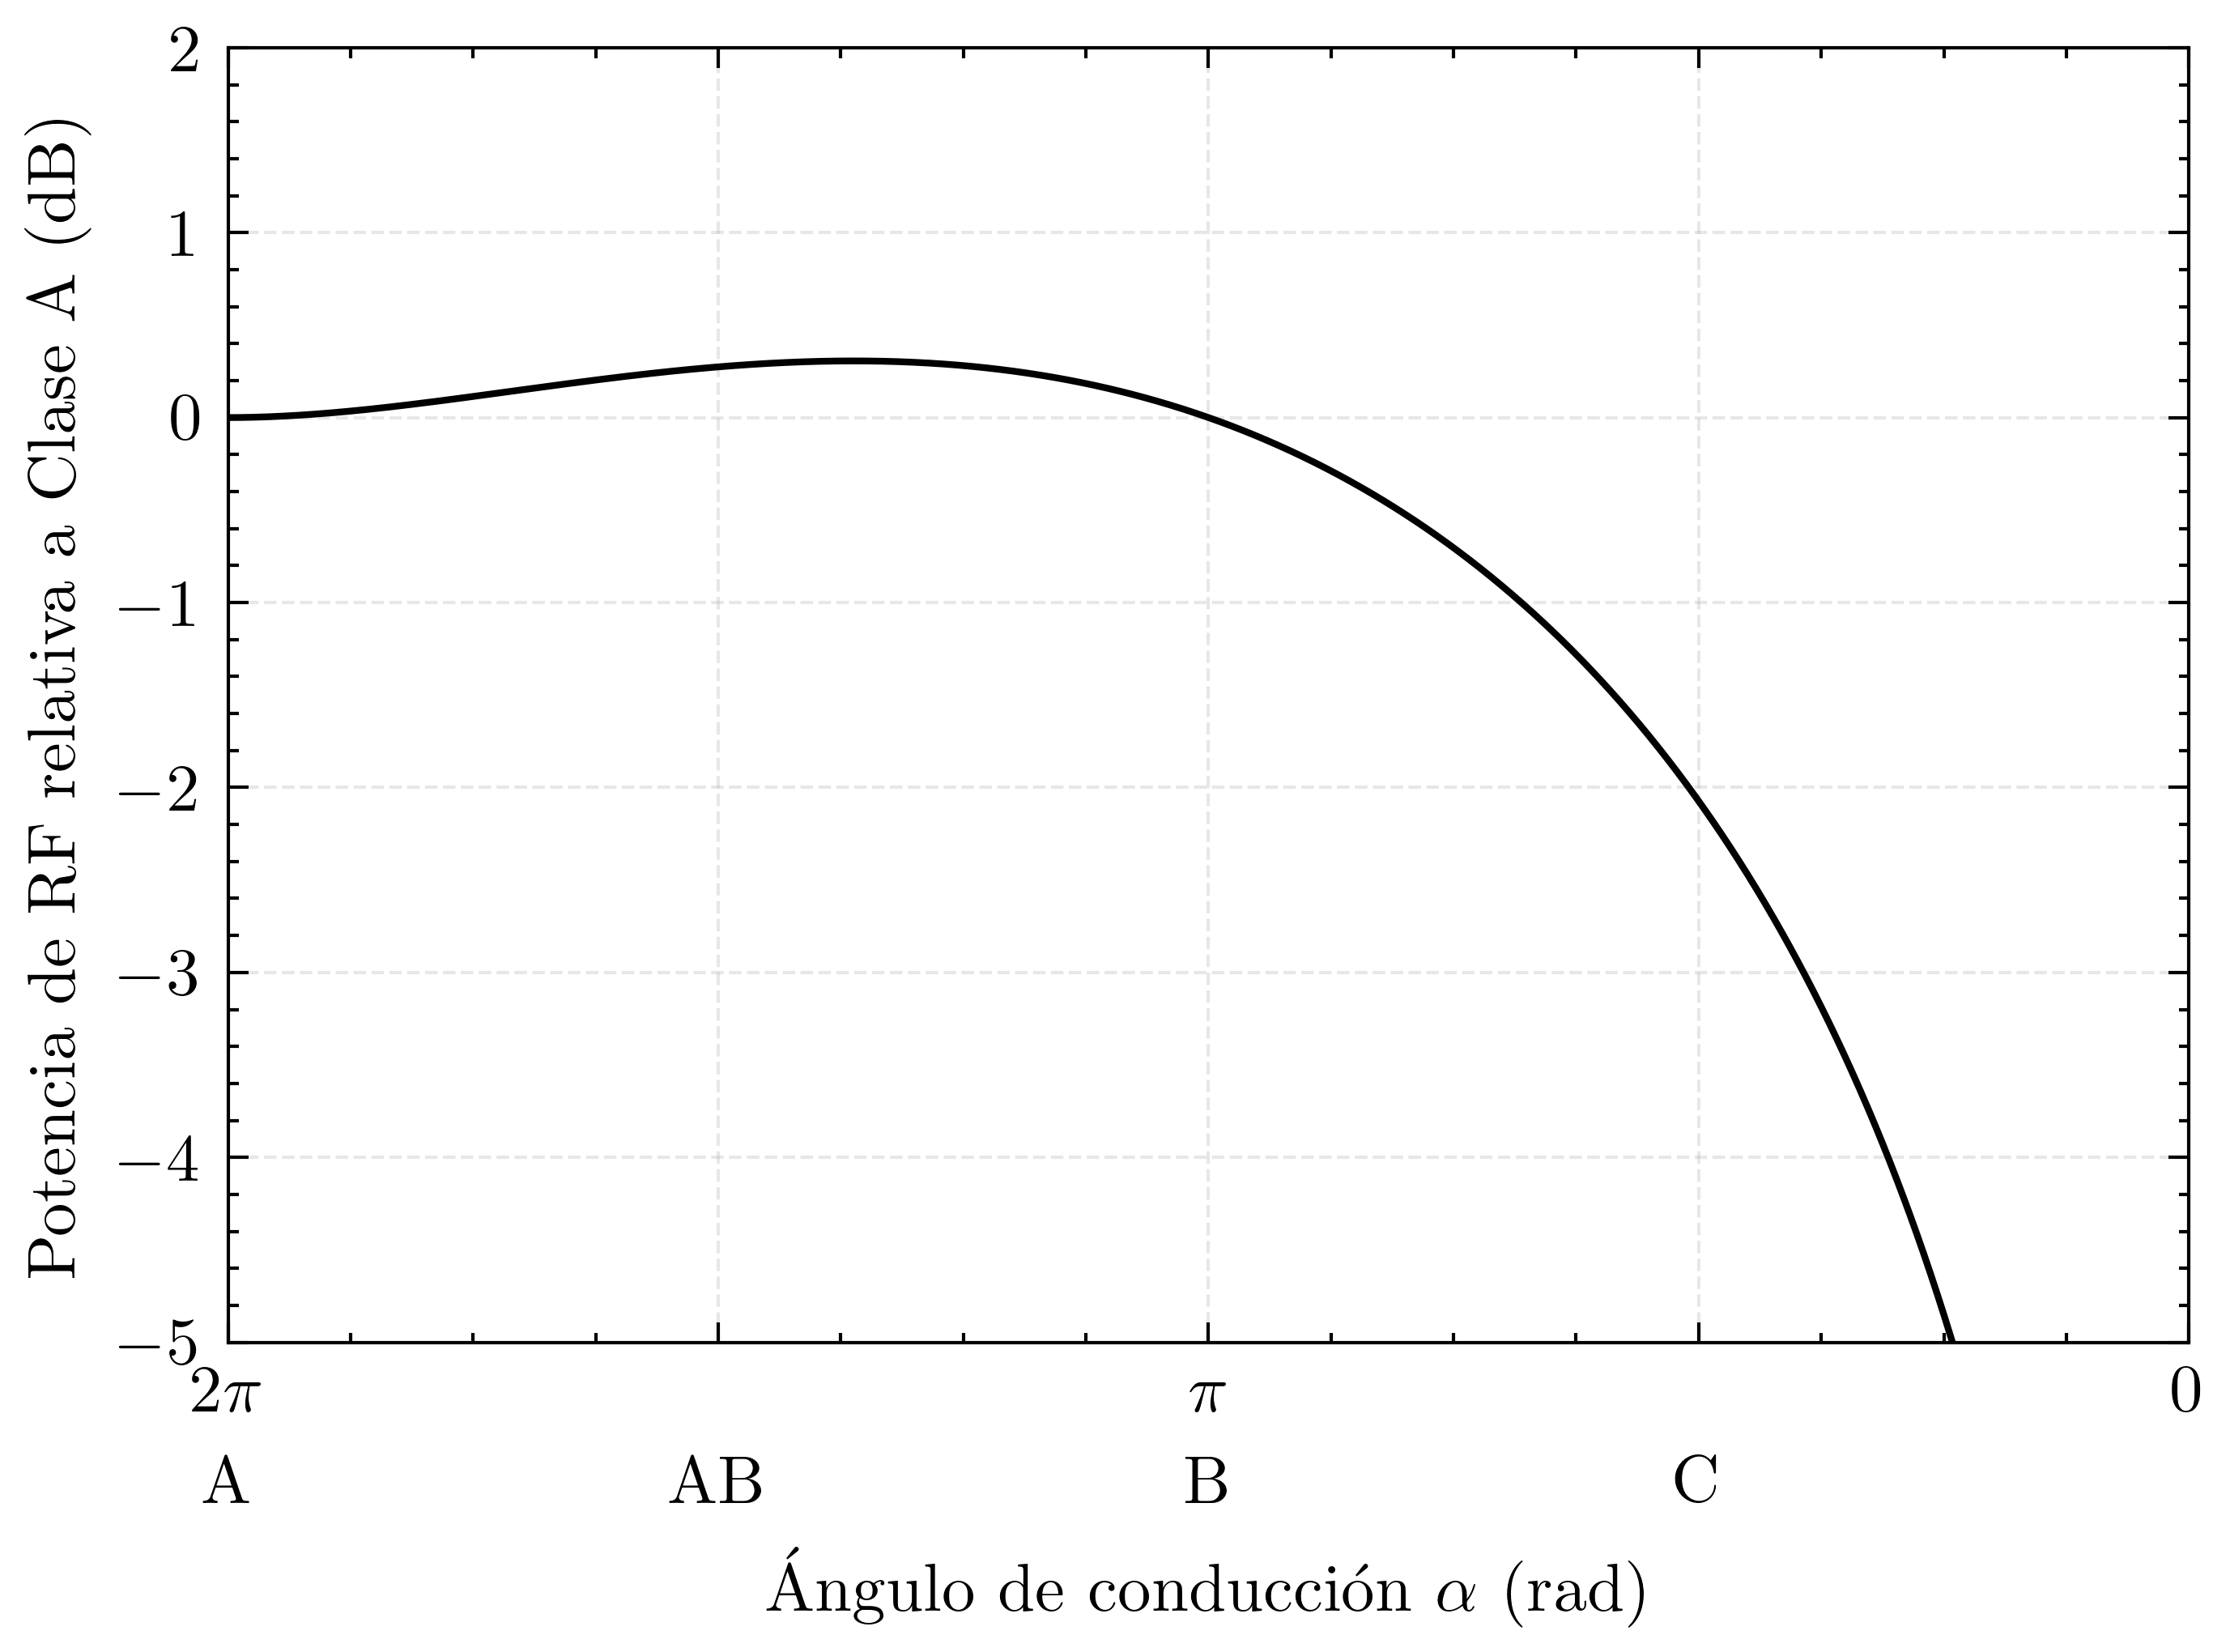
\includegraphics[width=0.85\linewidth]{Figures/rf_power.png}
    \caption{Potencia de RF entregada a la carga, relativa a Clase A, en función del ángulo de conducción, asumiendo carga óptima y cortocircuito en las frecuencias armónicas.}
    \label{fig:rf_power_alpha}
\end{figure}

% -----------------------------------------------------------------------------------------------%
\section{Parámetros de Pequeña Señal}
La caracterización de un amplificador de potencia en régimen de pequeña señal, es decir, con una excitación suficientemente pequeña como para que el dispositivo se comporte linealmente, se realiza mediante sus parámetros de dispersión o parámetros S \cite{kurokawa1965}. A diferencia de los parámetros de impedancia o admitancia, los parámetros S no relacionan tensiones y corrientes en los puertos del dispositivo, sino ondas de potencia incidentes y reflejadas, lo cual permite su medición directa a frecuencias de microondas sin requerir condiciones de circuito abierto o cortocircuito en los puertos, físicamente impracticables en esa banda de frecuencias.

Para un dispositivo de dos puertos como el transistor considerado (considerando el terminal de source conectado a masa), con el puerto de entrada asociado al terminal de gate y el puerto de salida asociado al terminal de drain, se definen las ondas de tensión normalizadas incidente ($a_i$) y reflejada ($b_i$) en cada puerto $i$, referidas a una impedancia característica $Z_0$, según se ilustra en la Figura~\ref{fig:cuadripolo_s}. Los cuatro parámetros S relacionan estas ondas mediante:

\begin{equation}
    \begin{pmatrix} b_1 \\ b_2 \end{pmatrix} =
    \begin{pmatrix} S_{11} & S_{12} \\ S_{21} & S_{22} \end{pmatrix}
    \begin{pmatrix} a_1 \\ a_2 \end{pmatrix}
    \label{eq:matriz_s}
\end{equation}

donde cada parámetro individual se obtiene, por definición, excitando un único puerto a la vez y colocando una carga adaptada en el puerto restante (de modo que la onda incidente en ese puerto sea nula), según:

\begin{equation}
    S_{11} = \frac{b_1}{a_1}\bigg|_{a_2 = 0} \quad
    S_{21} = \frac{b_2}{a_1}\bigg|_{a_2 = 0} \quad
    S_{12} = \frac{b_1}{a_2}\bigg|_{a_1 = 0} \quad
    S_{22} = \frac{b_2}{a_2}\bigg|_{a_1 = 0}
    \label{eq:definicion_s}
\end{equation}

El parámetro $S_{11}$ corresponde al coeficiente de reflexión en el puerto de entrada con el puerto de salida adaptado, y cuantifica la fracción de la onda incidente en el gate que es reflejada hacia la fuente de excitación. De manera análoga, $S_{22}$ corresponde al coeficiente de reflexión en el puerto de salida con la entrada adaptada, y cuantifica la fracción de potencia reflejada desde el drain hacia la carga. Ambos parámetros son magnitudes complejas adimensionales cuyo módulo, idealmente nulo en una condición de adaptación perfecta y de valor unitario en el caso de una reflexión total, determina directamente el desempeño de adaptación de impedancia del dispositivo en cada puerto.

El parámetro $S_{21}$ corresponde al coeficiente de transmisión directa, desde el puerto de entrada hacia el puerto de salida, y representa la ganancia del dispositivo en la condición de adaptación impuesta. El parámetro $S_{12}$ corresponde al coeficiente de transmisión inversa, desde el puerto de salida hacia el puerto de entrada, y cuantifica la magnitud de la realimentación interna del dispositivo. Un mayor valor de $S_{12}$ indica una realimentación interna mayor del dispositivo, factor que condiciona directamente la estabilidad del amplificador frente a variaciones en las impedancias de fuente y carga, según se desarrolla en la subsección siguiente.

\subsection{Factor de Estabilidad}
A partir de los parámetros S se evalúa la estabilidad del dispositivo, propiedad que determina si el amplificador es susceptible de entrar en oscilación para alguna combinación de impedancias de fuente y carga. Un dispositivo se clasifica como \textbf{incondicionalmente estable} para una frecuencia dada cuando permanece estable para cualquier combinación posible de impedancias de fuente y carga, es decir, para la totalidad del diagrama de Smith. Por el contrario, un dispositivo se clasifica como \textbf{condicionalmente estable} cuando existen regiones dentro del diagrama de Smith, denominadas regiones de inestabilidad, para las cuales alguna combinación de impedancias provoca que el dispositivo oscile. En este último caso, el diseñador debe restringir las impedancias de las redes de adaptación a las regiones estables identificadas mediante los círculos de estabilidad correspondientes.

El criterio de estabilidad más extendido es el factor de Rollet ($K$) \cite{rollet1962}, el cual, junto con la condición adicional sobre el determinante $|\Delta| < 1$ (donde $\Delta = S_{11}S_{22} - S_{12}S_{21}$), garantiza estabilidad incondicional cuando $K > 1$. Sin embargo, el presente trabajo prioriza el empleo del factor $\mu$ de Edwards-Sinsky como criterio de estabilidad \cite{edwards1992}, definido como:

\begin{equation}
    \mu = \frac{1 - |S_{11}|^2}{|S_{22} - S_{11}^{*}\Delta| + |S_{12}S_{21}|}
    \label{eq:mu_factor}
\end{equation}

El factor $\mu$ resulta preferible al factor $K$ de Rollet por dos motivos. En primer lugar, la condición $\mu > 1$ es necesaria y suficiente por sí sola para garantizar la estabilidad incondicional del dispositivo, sin requerir la verificación simultánea de una segunda condición sobre $\Delta$ como ocurre con el criterio de $K$. En segundo lugar, el valor numérico de $\mu$ constituye una medida directa del margen de estabilidad del dispositivo. Valores de $\mu$ progresivamente mayores a la unidad indican una mayor distancia respecto de la condición límite de inestabilidad, mientras que el factor $K$ no admite esta interpretación cuantitativa de manera tan directa. Ambos factores son calculados a partir de los parámetros S medidos o simulados, por lo cual resultan complementarios y consistentes entre sí.

\subsection{Ganancia de Potencia en Pequeña Señal}
La ganancia de un amplificador de potencia relaciona la potencia entregada a la carga con la potencia disponible en la fuente de excitación. En el caso general, en el cual las impedancias de generador ($Z_g$) y carga ($Z_L$) no coinciden necesariamente con la impedancia característica $Z_0$ empleada para definir los parámetros S, la ganancia de transducción (\textit{transducer power gain}, $G_T$) se define como el cociente entre la potencia efectivamente entregada a la carga y la potencia disponible de la fuente \cite[p.~561]{pozar2011}:

\begin{equation}
    G_T = \frac{|S_{21}|^2\,(1-|\Gamma_S|^2)(1-|\Gamma_L|^2)}{|1-\Gamma_S\Gamma_{in}|^2\,|1-S_{22}\Gamma_L|^2}
    \label{eq:ganancia_transductora}
\end{equation}

donde $\Gamma_S$ y $\Gamma_L$ son los coeficientes de reflexión de la fuente y de la carga, respectivamente, referidos a $Z_0$, y $\Gamma_{in}$ es el coeficiente de reflexión visto hacia la entrada del dispositivo con la carga $\Gamma_L$ conectada en su puerto de salida, dado por \cite[p.~560]{pozar2011}

\begin{equation}
    \Gamma_{in} = S_{11} + \frac{S_{12}S_{21}\Gamma_L}{1-S_{22}\Gamma_L}
    \label{eq:gamma_in}
\end{equation}

En el caso particular en que tanto la fuente como la carga se encuentran adaptadas a $Z_0$ ($\Gamma_S = \Gamma_L = 0$), la ecuación~\eqref{eq:ganancia_transductora} se reduce a:

\begin{equation}
    G_T\big|_{\Gamma_S=\Gamma_L=0} = |S_{21}|^2
    \label{eq:ganancia_s21}
\end{equation}

esta magnitud constituye la ganancia de pequeña señal del amplificador reportada habitualmente en las hojas de datos del fabricante y obtenida directamente a partir de la medición de parámetros S. Esta ganancia constituye una referencia de diseño relevante, dado que establece el límite superior de ganancia del dispositivo en la condición de excitación reducida, valor que, como se describe en la sección siguiente, decrece progresivamente a medida que el nivel de excitación se incrementa y el amplificador ingresa en su régimen de operación de gran señal.

% -----------------------------------------------------------------------------------------------%
\section{Parámetros de Gran Señal}
Los parámetros de pequeña señal descriptos en la sección anterior caracterizan al amplificador únicamente en la región donde su comportamiento puede aproximarse como lineal. Sin embargo, un amplificador de potencia se diseña precisamente para operar con niveles de excitación elevados, en los cuales el dispositivo abandona progresivamente dicha región lineal a medida que se aproxima a su punto de saturación. En estas condiciones, magnitudes como la ganancia dejan de ser constantes y pasan a depender del nivel de potencia de entrada, por lo cual la caracterización de pequeña señal resulta insuficiente para predecir el desempeño real del amplificador en su punto de operación de interés. Resulta entonces necesario definir un conjunto de parámetros adicionales, evaluados en régimen de gran señal, que permitan cuantificar tanto la potencia de salida alcanzable como la eficiencia con la cual dicha potencia es generada.

La \textbf{potencia de salida} ($P_{out}$) del amplificador, generalmente especificada en algún punto particular de la curva de transferencia de potencia según el contexto de diseño, constituye, junto con la eficiencia, uno de los parámetros centrales para la evaluación de cualquier sistema de comunicaciones de radiofrecuencia. La \textbf{potencia de saturación} ($P_{sat}$) corresponde al nivel máximo de potencia de salida que el dispositivo es capaz de entregar, independientemente del incremento adicional que se aplique al nivel de excitación de entrada. Este límite se debe a que la excursión de tensión y corriente en el drain del transistor se encuentra físicamente acotada por la tensión de alimentación y por la corriente máxima que el dispositivo admite. Incrementos adicionales en la potencia de entrada no se traducen en incrementos de la potencia de salida.

La \textbf{ganancia} del amplificador en régimen de gran señal, definida como el cociente entre la potencia de salida y la potencia de entrada, se mantiene aproximadamente constante mientras el dispositivo opera en la región lineal. A medida que la potencia de entrada se incrementa y el amplificador se aproxima a la saturación, la ganancia decrece. El \textbf{punto de compresión de 1 dB} (P1dB) constituye una de las figuras de mérito más relevantes de un amplificador de potencia, definido como el nivel de potencia de entrada para el cual la potencia de salida se aparta en 1 dB de la respuesta lineal extrapolada a partir del comportamiento de pequeña señal. Este punto marca, en consecuencia, el límite de la región de operación lineal del amplificador \cite[pp.~512--513]{pozar2011}.

Un valor de P1dB elevado indica que el amplificador puede entregar una mayor potencia de salida antes de que su comportamiento se aparte significativamente de la linealidad, deseable en aplicaciones que emplean esquemas de modulación con envolvente no constante, dado que las variaciones de amplitud de la señal deben amplificarse sin introducir distorsión apreciable para evitar la degradación de la calidad de la comunicación. En la práctica, rara vez opera el amplificador exactamente en su punto de saturación, sino que reserva un margen de \textit{backoff} respecto del P1dB, de modo de garantizar un margen adicional de linealidad frente a variaciones de la señal de entrada, aspecto que se retoma con mayor detalle en la Sección~\ref{sec:linealidad}. El P1dB se ubica siempre por debajo de la potencia de saturación, dado que la curva de transferencia de potencia continúa incrementándose más allá del punto de compresión, aunque con ganancia decreciente, hasta saturarse.

\begin{figure}[H]
    \centering
    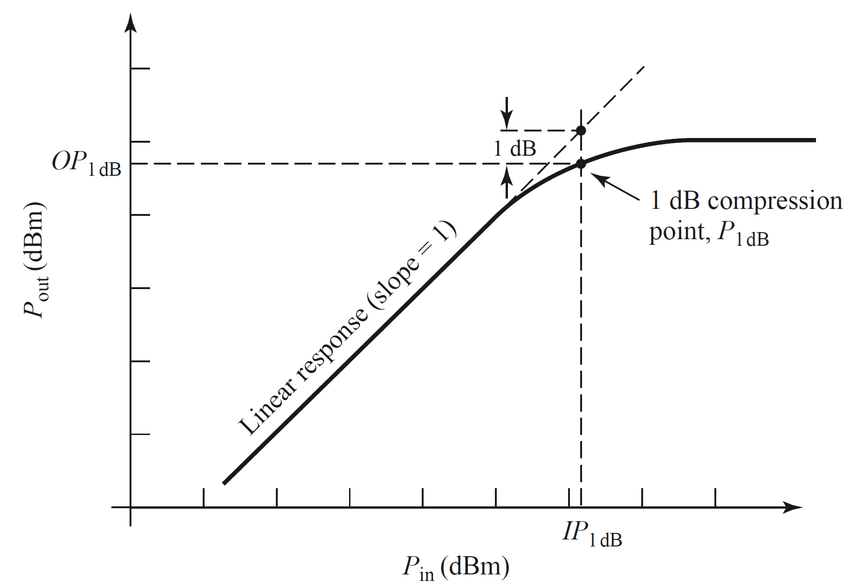
\includegraphics[width=0.8\linewidth]{Figures/p1dB_theory.png}
    \caption{Curva teórica del punto de compresión de 1\,dB \cite{taranto2020}.}
    \label{fig:p1db_theory}
\end{figure}

La \textbf{eficiencia de drain} ($\eta_D$) y la \textbf{eficiencia de potencia agregada} (\textit{power-added efficiency}, PAE) cuantifican la fracción de la potencia continua consumida que se convierte en potencia de RF y la fracción de potencia continua que se convierte en ganancia neta de potencia de radiofrecuencia, descontando la potencia de excitación entregada por la fuente de señal, respectivamente.

\begin{equation}
    \eta_D = \frac{P_{RF,out}}{P_{DC}}, \qquad \text{PAE} = \frac{P_{RF,out} - P_{RF,in}}{P_{DC}}
    \label{eq:pae_definicion}
\end{equation}

de modo que la PAE resulta siempre menor o igual a la eficiencia de drain, diferenciándose de manera apreciable únicamente en amplificadores de ganancia reducida, en los cuales la potencia de excitación de entrada deja de ser despreciable respecto de la potencia de salida. Ambas magnitudes dependen del nivel de excitación aplicado, y se evalúan habitualmente en el punto de compresión de 1 dB o en saturación, según el criterio de diseño adoptado, dado que es precisamente en las proximidades de dicho régimen donde el amplificador opera con la eficiencia más elevada, como se desprende del análisis de las clases de operación desarrollado en la Sección~\ref{sec:funcionamiento_clases}.

% -----------------------------------------------------------------------------------------------%
\section{Linealidad} \label{sec:linealidad}
El comportamiento de un amplificador de potencia frente a distintos niveles de excitación puede dividirse conceptualmente en dos regímenes de operación. En la \textbf{región lineal}, correspondiente a niveles de potencia de entrada sensiblemente inferiores al P1dB, la potencia de salida crece proporcionalmente con la potencia de entrada y la ganancia permanece aproximadamente constante e igual a su valor de pequeña señal. A medida que el nivel de excitación se incrementa y el amplificador se aproxima a la saturación, ingresa en la \textbf{región de compresión}, en la cual la ganancia decrece progresivamente y la relación entre potencia de entrada y de salida deja de ser lineal, hasta alcanzar asintóticamente la potencia de saturación descripta en la sección anterior.

Como ya se ha mencionado, el diseñador enfrenta un compromiso directo entre potencia de salida, eficiencia y linealidad. La práctica habitual para resolver este compromiso consiste en operar el amplificador con un cierto backoff, de modo de recuperar un margen de linealidad a costa de una eficiencia inferior. La magnitud del backoff depende de las características de la señal a amplificar, siendo particularmente relevante en esquemas de modulación con envolvente no constante, en los cuales las variaciones instantáneas de amplitud de la señal exigen que el amplificador permanezca en su región lineal incluso durante los picos de potencia de la envolvente.

\subsection{Distorsión Armónica}
Una primera manifestación de la no linealidad del amplificador es la distorsión armónica, ya introducida en la Sección~\ref{sec:funcionamiento_clases} al analizar la corriente de drain en función del ángulo de conducción. Dado que la relación entre la tensión aplicada en el gate y la corriente resultante en el drain no es lineal, una excitación de entrada puramente senoidal da origen, a la salida, a componentes en frecuencias múltiplos de la fundamental, según se desprende del desarrollo en serie de Fourier de la ecuación~\eqref{eq:fourier}. La magnitud relativa de estas componentes armónicas, ya cuantificada en la Figura~\ref{fig:armonicos_alpha} en función del ángulo de conducción, constituye una primera medida de la linealidad del dispositivo, aunque resulta insuficiente para caracterizar el comportamiento del amplificador frente a señales moduladas, dado que estas ocupan una banda de frecuencias en torno a la portadora en lugar de un único tono.

\subsection{Productos de Intermodulación y Prueba de Dos Tonos}
Cuando la señal de entrada del amplificador contiene más de una componente frecuencial, la no linealidad del dispositivo no solo genera armónicos de cada componente individual, sino también productos de intermodulación, es decir, componentes espectrales adicionales ubicadas en combinaciones lineales de las frecuencias originales. Este comportamiento resulta de particular relevancia, por ejemplo, para señales moduladas digitalmente, que ocupan una banda de frecuencias en torno a la portadora, por lo que las distintas componentes frecuenciales interactúan entre sí, generando productos de intermodulación que caen dentro o en las proximidades de la banda de interés y que no pueden eliminarse mediante filtrado posterior.

Para analizar el origen de estos productos, la característica de transferencia no lineal del amplificador puede aproximarse mediante un desarrollo en serie de potencias de la tensión de entrada $v_{in}(t)$, truncado hasta el tercer orden \cite[pp.~233--240]{cripps2006}

\begin{equation}
    v_{out}(t) = a_1\,v_{in}(t) + a_2\,v_{in}^2(t) + a_3\,v_{in}^3(t)
    \label{eq:serie_potencias}
\end{equation}

donde $a_1$ representa la ganancia lineal del amplificador, y los coeficientes $a_2$ y $a_3$ cuantifican, respectivamente, el grado de no linealidad de segundo y tercer orden de la característica de transferencia. La \textbf{prueba de dos tonos} consiste en excitar al amplificador con dos señales senoidales de igual amplitud $A$ y frecuencias cercanas entre sí, de modo que:

\begin{equation}
    v_{in}(t) = A\cos(\omega_1 t) + A\cos(\omega_2 t)
    \label{eq:dos_tonos}
\end{equation}

Sustituyendo la ecuación~\eqref{eq:dos_tonos} en~\eqref{eq:serie_potencias} y desarrollando mediante identidades trigonométricas, se obtiene un conjunto de componentes espectrales en distintas combinaciones de $\omega_1$ y $\omega_2$. Entre ellas, el término $a_3\,v_{in}^3(t)$ da origen, en particular, a componentes en las frecuencias $2\omega_1 - \omega_2$ y $2\omega_2 - \omega_1$, cuya amplitud resulta

\begin{equation}
    A_{IM3} = \frac{3}{4}\,a_3\,A^3
    \label{eq:amplitud_im3}
\end{equation}

mientras que la amplitud de la componente fundamental, considerando la contribución del término cúbico sobre la propia frecuencia de excitación, resulta:

\begin{equation}
    A_{fund} = a_1\,A + \frac{9}{4}\,a_3\,A^3 \approx a_1\,A
    \label{eq:amplitud_fund}
\end{equation}

donde la aproximación es válida en la región de operación de interés, en la cual el término lineal domina sobre la contribución de tercer orden. Entre los productos de intermodulación generados, los ubicados en $2f_1 - f_2$ y $2f_2 - f_1$ son los de mayor interés práctico, dado que se encuentran próximos a las frecuencias originales y, por lo tanto, no pueden ser removidos mediante filtrado sin afectar también a la señal deseada. Los productos de intermodulación de orden par, en cambio, aparecen alejados de la banda de interés y resultan de menor relevancia práctica en la mayoría de las aplicaciones de comunicaciones. En la Figura~\ref{fig:im_spectrum} se ilustran los productos de intermodulación cercanos a las frecuencia de los tonos.

\begin{figure}[H]
    \centering
    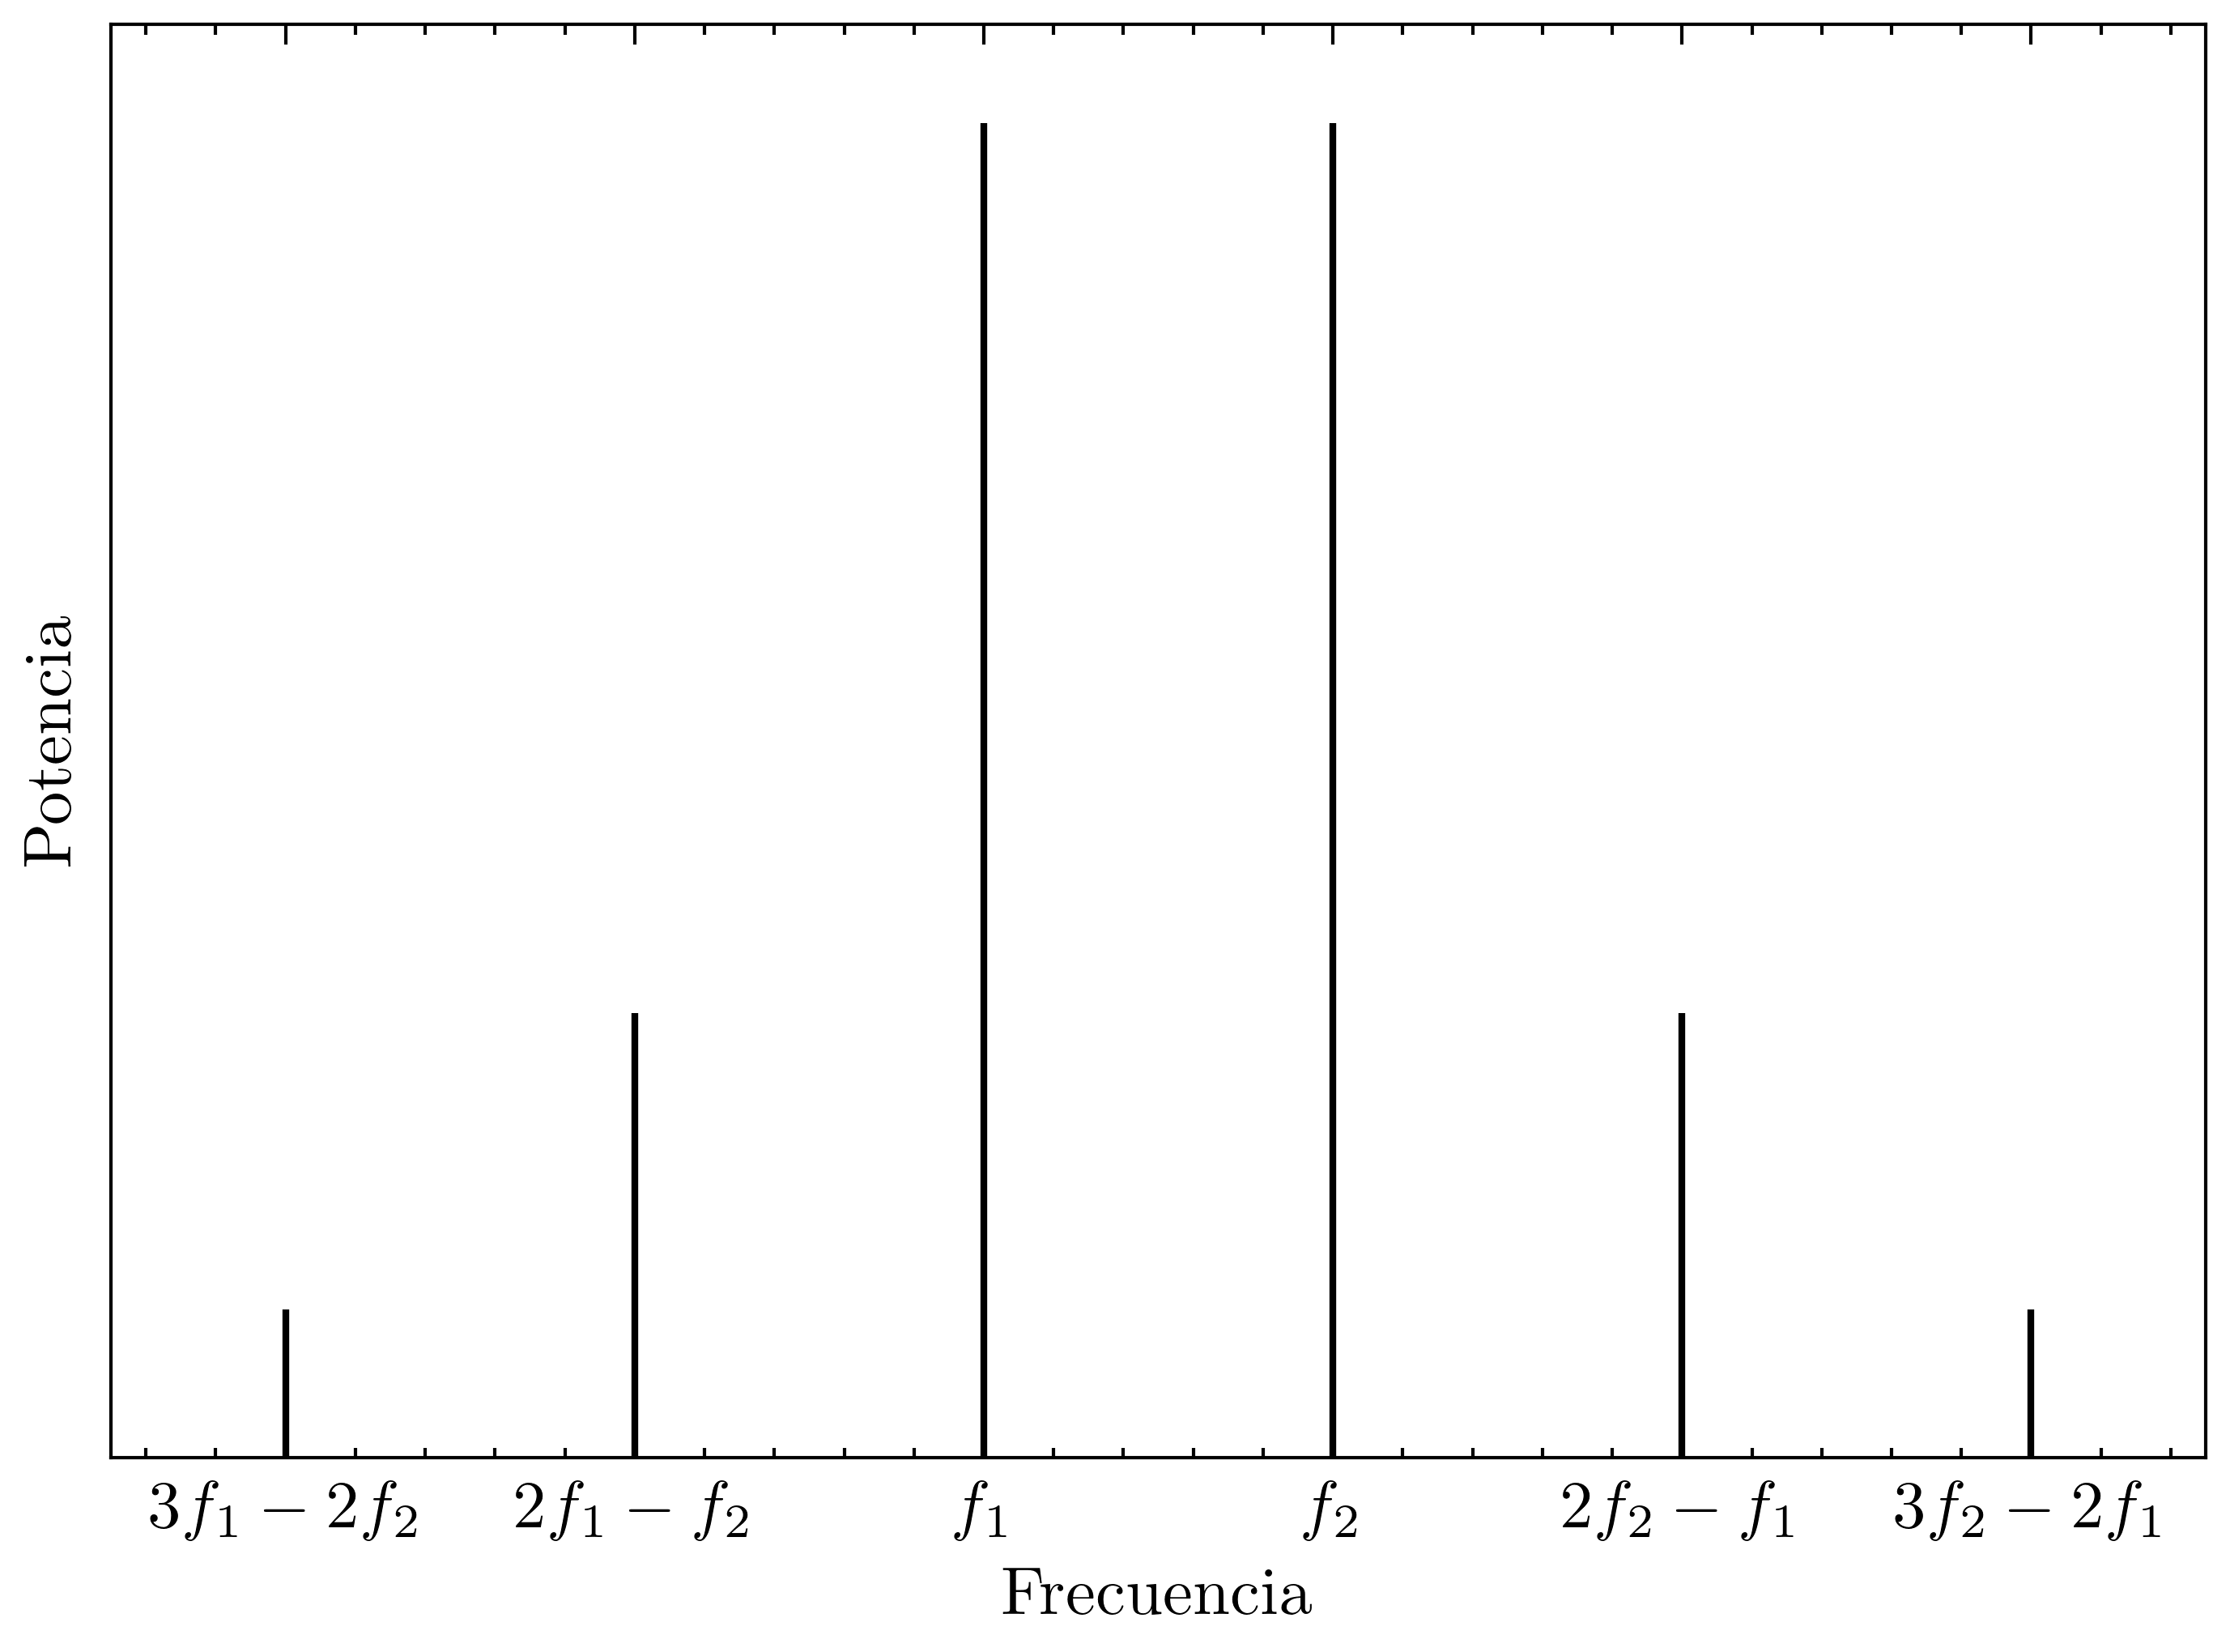
\includegraphics[width=0.7\linewidth]{Figures/im_spectrum.png}
    \caption{Productos de intermodulación cercanos a las frecuencias de los tonos de la señal de entrada.}
    \label{fig:im_spectrum}
\end{figure}

De las ecuaciones~\eqref{eq:amplitud_im3} y \eqref{eq:amplitud_fund} se desprende que, en la región donde ambas aproximaciones resultan válidas, la potencia de la componente fundamental ($P_{fund} \propto A_{fund}^2 \propto A^2$) crece con una pendiente de 1 dB por cada dB de incremento en la potencia de entrada, mientras que la potencia de los productos de intermodulación de tercer orden ($P_{IM3} \propto A_{IM3}^2 \propto A^6$) crece con una pendiente de 3 dB por dB, dado que su amplitud resulta proporcional a $A^3$. Expresando ambas magnitudes en escala logarítmica, la potencia fundamental y la potencia de los productos de tercer orden pueden aproximarse mediante dos rectas de pendiente 1 y 3 respectivamente, en función de la potencia de entrada expresada en dBm. Estas rectas, extrapoladas más allá de la región donde la aproximación de la ecuación~\eqref{eq:serie_potencias} deja de ser válida, se interceptan en un punto teórico denominado \textbf{punto de intercepción de tercer orden} (IP3), definido formalmente como el nivel de potencia hipotético para el cual la potencia extrapolada de la componente fundamental es igual a la de los productos de intermodulación de tercer orden \cite[pp.~515--517]{pozar2011}. Este punto puede referirse tanto a la entrada del amplificador (\textit{Input IP3}, IIP3) como a su salida (\textit{Output IP3}, OIP3), siendo esta última la magnitud más utilizada en la práctica. El IP3 constituye un valor teórico que no es físicamente alcanzable por el dispositivo, dado que ambas curvas se saturan antes de alcanzar dicho punto, pero resulta una figura de mérito estándar para comparar la linealidad de distintos amplificadores de manera independiente del nivel de potencia de excitación empleado durante el ensayo.

\begin{figure}[H]
    \centering
    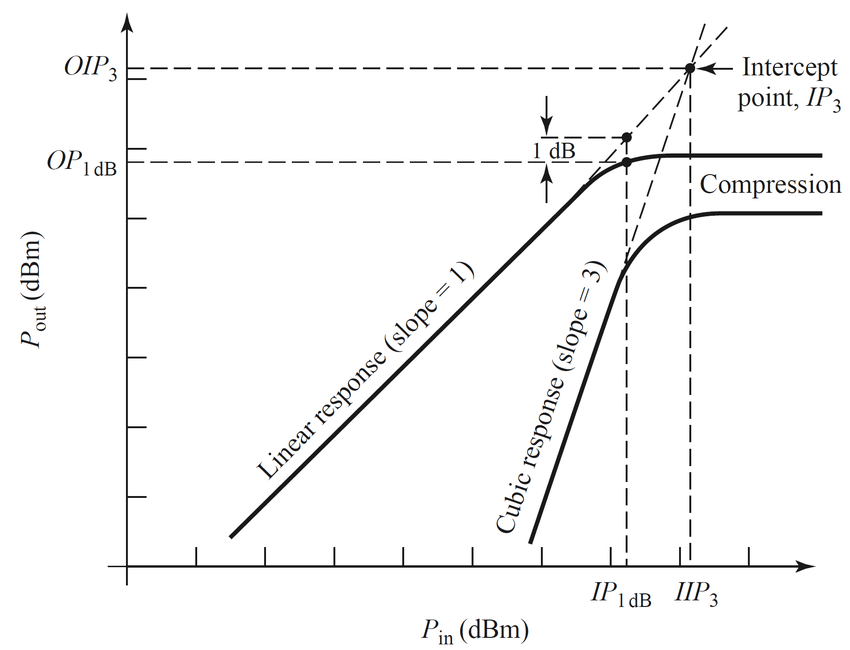
\includegraphics[width=0.8\linewidth]{Figures/oip3_theory.png}
    \caption{Curva teórica del punto de intercepción de tercer orden referido a la salida y del punto de compresión de 1\,dB \cite{taranto2020}.}
    \label{fig:oip3_theory}
\end{figure}

En \cite{cripps2006} se señala que, el OIP3 se relaciona empíricamente con el P1dB mediante un factor aproximadamente constante, de modo que

\begin{equation}
    OIP3 \approx P_{1dB} + 10 \text{ dB}
    \label{eq:oip3_p1db}
\end{equation}

Esta relación empírica resulta de utilidad práctica, dado que permite estimar una figura de mérito de linealidad frente a señales de banda ancha (OIP3) a partir de una medición de compresión de ganancia mucho más simple de realizar (P1dB), sin necesidad de efectuar el ensayo de dos tonos completo en las etapas preliminares del diseño.

\subsection{Conversión AM-PM}
Otro fenómeno no lineal, menos intuitivo que los descriptos anteriormente, presente en amplificadores de potencia es la conversión AM-PM, donde variaciones en la amplitud de la señal de entrada provocan una variación en la fase de la señal presente a la salida. De esta definición puede comenzar a intuirse la importancia de mitigar este efecto en sistemas digitales que emplean un esquema de modulación de fase o frecuencia, dado que dicha variación de fase inducida por la amplitud degrada directamente la información transmitida.

Este fenómeno no se manifiesta en el modelo de no linealidad empleado hasta aquí, en el cual la respuesta del dispositivo en cada instante depende únicamente del valor instantáneo de la tensión de entrada. Bajo dicho modelo, las componentes de primer y tercer orden se encuentran en fase entre sí, de modo que un incremento en la amplitud de la señal de entrada modifica únicamente la amplitud a la salida, sin introducir variación alguna en su fase \cite[pp.15--16]{maas2003}.

En un dispositivo real, sin embargo, las alinealidades del transistor presentan un comportamiento reactivo asociado a capacitancias del dispositivo. Bajo estas condiciones, la componente de tercer orden no se encuentra necesariamente en fase con la componente lineal, de modo que la respuesta a la frecuencia fundamental debe expresarse como la suma fasorial de ambas componentes.

Aun con un desfasaje constante, la fase resultante varía con la amplitud de la excitación, dado que la suma fasorial entre un término de amplitud constante en fase y un término de amplitud creciente con la tercera potencia de $V_1$ y fase distinta modifica el ángulo de la resultante a medida que $V_1$ se incrementa. Este comportamiento constituye precisamente la conversión AM-PM, cuyo efecto se acentúa a medida que el dispositivo se aproxima a su región de saturación, dado que es en dicha región donde la contribución del término de tercer orden respecto del término lineal se torna más significativa .

% -----------------------------------------------------------------------------------------------%
\section{Diseño y Optimización de Amplificadores de Potencia}
El diseño de la etapa de amplificación no se limita a la selección del transistor y de su punto de polarización, sino que requiere adicionalmente el diseño de las redes de adaptación de impedancia que vinculan al dispositivo con la fuente de excitación y con la carga. La \textbf{adaptación de impedancia} consiste en interponer, entre dos puertos de impedancias distintas, una red circuital, típicamente reactiva e idealmente sin pérdidas, que transforma una de dichas impedancias en el conjugado complejo de la otra, o bien en algún otro valor de interés según el criterio adoptado, con el objetivo de controlar la transferencia de potencia entre ambos puertos \cite[Cap.~5]{pozar2011}.

\subsection{Adaptación de Entrada}
En el puerto de entrada del amplificador, el objetivo de diseño es maximizar la transferencia de potencia disponible desde la fuente de excitación hacia el gate del transistor. Este objetivo se alcanza mediante el teorema de máxima transferencia de potencia, según el cual la potencia entregada a una carga es máxima cuando la impedancia de dicha carga es igual al complejo conjugado de la impedancia de la fuente que la excita \cite[pp-76--78]{pozar2011}. Aplicado al puerto de entrada del amplificador, esto implica diseñar la red de adaptación de entrada de modo que la impedancia que ve el generador sea igual al conjugado complejo de la impedancia de fuente $Z_g$, es decir, $Z_{in} = Z_g^*$. Dado que en el puerto de entrada el objetivo es únicamente maximizar la potencia entregada al dispositivo sin que existan consideraciones adicionales de gran señal, la adaptación conjugada resulta el criterio de diseño apropiado y suficiente para esta red.

\subsection{Adaptación de Salida}
El criterio de adaptación conjugada, sin embargo, no resulta aplicable de la misma manera en el puerto de salida del amplificador. El teorema de máxima transferencia de energía considera a un generador ideal, sin límites físicos de tensión y corriente en sus terminales, restricción que resulta determinante cuando dicho generador es la fuente de corriente de salida de un transistor de potencia \cite[pp.11--14]{cripps2006}.

Tomando el ejemplo de \cite[p.~12]{cripps2006}, y expandiendo sobre este, consideremos un transistor cuya salida se modela como una fuente de corriente con $I_{max}=1$~A en paralelo con una resistencia interna $R_{gen}=100\,\Omega$. Aplicando el criterio de adaptación conjugada, colocamos una carga $R_{load}=100\,\Omega$, resistencia que, en paralelo con $R_{gen}$, presenta una resistencia efectiva de $50\,\Omega$ a la fuente de corriente. En consecuencia, cuando la corriente alcanza su valor máximo de 1~A, la tensión resultante en los terminales del generador asciende a 50~V, valor que muy probablemente exceda la tensión que el dispositivo real es capaz de sostener, ya sea por su tensión de ruptura o por la tensión de alimentación disponible. Como consecuencia, el transistor entra en compresión a un nivel de corriente sustancialmente inferior a su capacidad física $I_{max}$, sin llegar a aprovechar la totalidad de la excursión de corriente disponible del dispositivo. Si la tensión de alimentación máxima es $V_{DD}=30\,V$ la corriente máxima que puede entregarse será de $0{,}6~\,A$ en lugar de $1~\,A$.

Para evitar esta limitación y aprovechar la excursión completa de tensión y corriente que el transistor es capaz de entregar, resulta necesario seleccionar, en cambio, una resistencia de carga menor que la conjugada, denominada resistencia de \textbf{loadline}, dada aproximadamente por:

\begin{equation}
    R_{opt} \approx \frac{V_{max}}{I_{max}}
    \label{eq:rl_optima}
\end{equation}

donde $V_{max}$ es la máxima tensión que el dispositivo admite en su terminal de drain, e $I_{max}$ es la corriente máxima de drain. Esta relación no contradice el teorema de máxima transferencia de potencia, sino que constituye un compromiso adicional propio del caso real, en el cual dicho teorema se aplica sujeto a las restricciones físicas de tensión y corriente del dispositivo.

Existe, además, una razón adicional por la cual el criterio de adaptación conjugada pierde sentido en el diseño de la red de salida de un amplificador de potencia. Un dispositivo que opera en Clase A, sin recorte de la forma de onda de corriente, presenta efectivamente una impedancia de salida aproximadamente constante a lo largo del ciclo, cercana a la descripta por el parámetro $S_{22}$, de modo que su comportamiento resulta razonablemente compatible con un modelo de generador de Thevenin. Sin embargo, en un dispositivo que opera con ángulo de conducción reducido, como las Clases AB, B o C presentadas en la Sección~\ref{sec:funcionamiento_clases}, el transistor permanece en corte durante una porción del ciclo durante el cual no conduce corriente y presenta, por definición, un circuito abierto en su salida. En estas condiciones, la conductancia instantánea de salida del dispositivo varía a lo largo del ciclo en lugar de permanecer constante, de modo que el concepto mismo de una impedancia de salida fija, y por lo tanto de un valor conjugado bien definido, deja de tener sentido físico \cite[p.~13]{cripps2006}.

En consecuencia, la impedancia de carga óptima de un amplificador de potencia no puede obtenerse a partir de sus parámetros S de pequeña señal, sino que depende de los límites de excursión de tensión y corriente del dispositivo en régimen de gran señal, según se desprende de la ecuación~\eqref{eq:rl_optima}, y del comportamiento no lineal de su corriente de drain a lo largo del ciclo de conducción.

\subsection{Método de Load-Pull}
Dado que la expresión~\eqref{eq:rl_optima} constituye únicamente una aproximación, que no contempla efectos como las capacitancias parásitas, armónicos en la impedancia de carga ni las no linealidades de orden superior de la corriente de drain, la impedancia óptima empleada en el diseño práctico se determina habitualmente mediante la técnica de \textbf{load-pull}. Esta técnica consiste en variar la impedancia de carga presentada al puerto de salida del transistor, manteniendo fijo el nivel de excitación de entrada, y registrar en cada punto del barrido el desempeño resultante del dispositivo \cite[p.~598]{pozar2011}.

El resultado de un barrido de load-pull se representa habitualmente mediante contornos trazados sobre el diagrama de Smith, donde cada contorno conecta los puntos de impedancia de carga que producen un mismo valor de una magnitud de interés, típicamente la potencia de salida ($P_{out}$), como se muestra en la Figura~\ref{fig:load_pull_theory} o la eficiencia de potencia agregada (PAE). Estos contornos permiten identificar, para un nivel de excitación dado, la región del diagrama de Smith donde el dispositivo alcanza su máxima potencia de salida y la región donde alcanza su máxima eficiencia, regiones que, en general, no coinciden entre sí. La impedancia de carga de diseño se selecciona entonces como un compromiso entre ambos criterios, priorizando la intersección de los contornos donde ambas magnitudes se mantienen simultáneamente próximas a sus valores máximos, en lugar de optimizar exclusivamente alguna de las dos de forma aislada.

\begin{figure}[H]
    \centering
    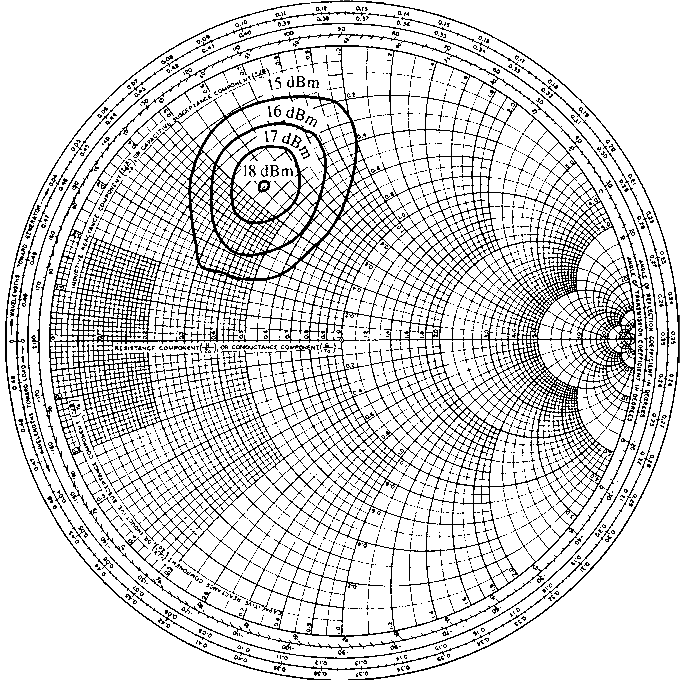
\includegraphics[width=0.8\linewidth]{Figures/load_pull_theory.png}
    \caption{Diagrama de Smith con contornos de impedancias para distintos valores de potencia de salida constante en un transistor de potencia\cite[p.~598]{pozar2011}.}
    \label{fig:load_pull_theory}
\end{figure}

\section{Conclusión}
A lo largo del capítulo se desarrollaron los fundamentos teóricos necesarios para abordar el diseño de un amplificador de potencia de RF. El análisis del ángulo de conducción permitió establecer que la clase de operación de un amplificador implica un compromiso entre eficiencia, potencia de salida y linealidad. 

Asimismo, se estableció que la caracterización de pequeña señal, si bien es necesaria para evaluar la estabilidad y la ganancia lineal del dispositivo, resultan insuficientes para predecir su comportamiento para los valores de excitación de interés. Los parámetros de gran señal compensan la carencia de los parámetros S, en particular el punto de compresión de 1 dB, la potencia de saturación y las distintas métricas de eficiencia, resultan indispensables para caracterizar el desempeño real del dispositivo en su punto de operación.

Por otra parte, se explicaron los mecanismos más relevantes que dan origen a la distorsión de la señal, estableciendo al OIP3 como figura de mérito y su vinculación empírica con el P1dB. Se destacó que la conversión AM-PM introduce distorsión adicional de particular relevancia para esquemas de modulación con envolvente no constante, como los empleados en el presente trabajo, dado que la variación de fase inducida por la amplitud de la señal degrada directamente la constelación recibida.

Finalmente, se discutió que el diseño de las redes de adaptación de impedancia no puede abordarse mediante un único criterio aplicable indistintamente a ambos puertos. Mientras que la adaptación de entrada admite el criterio de máxima transferencia de potencia, dicho criterio deja de ser válido en el puerto de salida. Por tal motivo, la adaptación de salida requiere de la determinación experimental o simulada de la impedancia óptima de carga mediante la técnica de load-pull.

En síntesis, el diseño de un amplificador de potencia constituye un problema de optimización de múltiples variables, en el cual la potencia de salida, la eficiencia, la linealidad y la estabilidad se encuentran acopladas, por ende ninguna de estas variables puede maximizarse sin afectar a las restantes. Los criterios y herramientas presentados en este capítulo constituyen el marco teórico sobre el cual se fundamentan las decisiones de diseño del amplificador desarrollado en capítulos posteriores.